\documentclass[11pt,a4paper]{article}
\usepackage{jheppub}
\pdfoutput=1
\toccontinuoustrue
\usepackage{lscape}
\usepackage{vruler}
\usepackage{subfigure}
\usepackage{appendix}

\newcommand{\blue}[1]{{\color{blue}{#1}\color{black}}}
\newcommand{\red}[1]{{\color{red}{#1}\color{black}}}

\def\desy{{\sc desy}}

\begin{document}
\title{Beam-Helicity and Beam-Charge Asymmetries \\
        in the Bethe-Heitler and DVCS processes on \\
        an Unpolarised Proton Target
  	\underline{Paper Tag: PDVCS0607 (v1.0)}
        \underline{Drafting Committee: DC90 (\today)}
}


% List of Institute Addresses 
\collaboration{The HERMES Collaboration}
\collaborationImg{
\includegraphics{hermeslogo.pdf}}

\author[12]{A.~Airapetian}
\author[26]{N.~Akopov}
\author[5]{Z.~Akopov}
\author[6]{E.C.~Aschenauer}
\author[25]{W.~Augustyniak}
\author[26]{R.~Avakian}
\author[26]{A.~Avetissian}
\author[5]{E.~Avetisyan}
\author[15]{B.~Ball}
\author[18]{S.~Belostotski}
\author[10]{N.~Bianchi}
\author[17,24]{H.P.~Blok}
\author[6]{H.~B\"ottcher}
\author[5]{A.~Borissov}
\author[13]{J.~Bowles}
\author[12]{I.~Brodski}
\author[19]{V.~Bryzgalov}
\author[13]{J.~Burns}
\author[9]{M.~Capiluppi}
\author[10]{G.P.~Capitani}
\author[21]{E.~Cisbani}
\author[9]{G.~Ciullo}
\author[9]{M.~Contalbrigo}
\author[9]{P.F.~Dalpiaz}
\author[5]{W.~Deconinck}
\author[2]{R.~De~Leo}
\author[5,22]{L.~De~Nardo}
\author[10]{E.~De~Sanctis}
\author[8]{M.~Diefenthaler}
\author[10]{P.~Di~Nezza}
\author[17]{J.~Dreschler}
\author[12]{M.~D\"uren}
\author[12]{M.~Ehrenfried}
\author[26]{G.~Elbakian}
\author[4]{F.~Ellinghaus}
\author[6]{R.~Fabbri}
\author[10]{A.~Fantoni}
\author[22]{L.~Felawka}
\author[21]{S.~Frullani}
\author[6]{D.~Gabbert}
\author[19]{G.~Gapienko}
\author[19]{V.~Gapienko}
\author[21]{F.~Garibaldi}
\author[5,18,22]{G.~Gavrilov}
\author[26]{V.~Gharibyan}
\author[9]{F.~Giordano}
\author[15]{S.~Gliske}
\author[5]{M.~Golembiovskaya}
\author[10]{C.~Hadjidakis}
\author[5]{M.~Hartig}
\author[10]{D.~Hasch}
\author[23]{T.~Hasegawa}
\author[13]{G.~Hill}
\author[6]{A.~Hillenbrand}
\author[13]{M.~Hoek}
\author[5]{Y.~Holler}
\author[6]{I.~Hristova}
\author[23]{Y.~Imazu}
\author[19]{A.~Ivanilov}
\author[18]{A.~Izotov}
\author[1]{H.E.~Jackson}
\author[18]{A.~Jgoun}
\author[11]{H.S.~Jo}
\author[14]{S.~Joosten}
\author[13]{R.~Kaiser}
\author[26]{G.~Karyan}
\author[12]{T.~Keri}
\author[4]{E.~Kinney}
\author[18]{A.~Kisselev}
\author[23]{N.~Kobayashi}
\author[19]{V.~Korotkov}
\author[16]{V.~Kozlov}
\author[18]{P.~Kravchenko}
\author[7]{V.G.~Krivokhijine}
\author[2]{L.~Lagamba}
\author[14]{R.~Lamb}
\author[17]{L.~Lapik\'as}
\author[13]{I.~Lehmann}
\author[9]{P.~Lenisa}
\author[14]{L.A.~Linden-Levy}
\author[11]{A.~L\'opez~Ruiz}
\author[15]{W.~Lorenzon}
\author[5]{X.-G.~Lu}
\author[23]{X.-R.~Lu}
\author[3]{B.-Q.~Ma}
\author[13]{D.~Mahon}
\author[14]{N.C.R.~Makins}
\author[18]{S.I.~Manaenkov}
\author[21]{L.~Manfr\'e}
\author[3]{Y.~Mao}
\author[25]{B.~Marianski}
\author[4]{A.~Martinez de la Ossa}
\author[26]{H.~Marukyan}
\author[22]{C.A.~Miller}
\author[23]{Y.~Miyachi}
\author[26]{A.~Movsisyan}
\author[10]{V.~Muccifora}
\author[13]{M.~Murray}
\author[8]{A.~Mussgiller}
\author[2]{E.~Nappi}
\author[18]{Y.~Naryshkin}
\author[8]{A.~Nass}
\author[6]{M.~Negodaev}
\author[6]{W.-D.~Nowak}
\author[9]{L.L.~Pappalardo}
\author[12]{R.~Perez-Benito}
\author[8]{N.~Pickert}
\author[8]{M.~Raithel}
\author[1]{P.E.~Reimer}
\author[10]{A.R.~Reolon}
\author[6]{C.~Riedl}
\author[8]{K.~Rith}
\author[13]{G.~Rosner}
\author[5]{A.~Rostomyan}
\author[14]{J.~Rubin}
\author[11]{D.~Ryckbosch}
\author[19]{Y.~Salomatin}
\author[20]{F.~Sanftl}
\author[20]{A.~Sch\"afer}
\author[11]{G.~Schnell}
\author[5]{K.P.~Sch\"uler}
\author[13]{B.~Seitz}
\author[23]{T.-A.~Shibata}
\author[7]{V.~Shutov}
\author[9]{M.~Stancari}
\author[9]{M.~Statera}
\author[8]{E.~Steffens}
\author[17]{J.J.M.~Steijger}
\author[12]{H.~Stenzel}
\author[6]{J.~Stewart}
\author[8]{F.~Stinzing}
\author[26]{S.~Taroian}
\author[16]{A.~Terkulov}
\author[25]{A.~Trzcinski}
\author[11]{M.~Tytgat}
\author[11]{A.~Vandenbroucke}
\author[17]{P.B.~van~der~Nat}
\author[11]{Y.~Van~Haarlem}
\author[11]{C.~Van~Hulse}
\author[5]{M.~Varanda}
\author[18]{D.~Veretennikov}
\author[18]{V.~Vikhrov}
\author[2]{I.~Vilardi}
\author[8]{C.~Vogel}
\author[3]{S.~Wang}
\author[8]{S.~Yaschenko}
\author[3]{H.~Ye}
\author[5]{Z.~Ye}
\author[22]{S.~Yen}
\author[12]{W.~Yu}
\author[8]{D.~Zeiler}
\author[5]{B.~Zihlmann}
\author[25]{P.~Zupranski}

\affiliation[1]{Physics Division, Argonne National Laboratory, Argonne, Illinois 60439-4843, USA}
\affiliation[2]{Istituto Nazionale di Fisica Nucleare, Sezione di Bari, 70124 Bari, Italy}
\affiliation[3]{School of Physics, Peking University, Beijing 100871, China}
\affiliation[4]{Nuclear Physics Laboratory, University of Colorado, Boulder, Colorado 80309-0390, USA}
\affiliation[5]{DESY, 22603 Hamburg, Germany}
\affiliation[6]{DESY, 15738 Zeuthen, Germany}
\affiliation[7]{Joint Institute for Nuclear Research, 141980 Dubna, Russia}
\affiliation[8]{Physikalisches Institut, Universit\"at Erlangen-N\"urnberg, 91058 Erlangen, Germany}
\affiliation[9]{Istituto Nazionale di Fisica Nucleare, Sezione di Ferrara and Dipartimento di Fisica, Universit\`a di Ferrara, 44100 Ferrara, Italy}
\affiliation[10]{Istituto Nazionale di Fisica Nucleare, Laboratori Nazionali di Frascati, 00044 Frascati, Italy}
\affiliation[11]{Department of Subatomic and Radiation Physics, University of Gent, 9000 Gent, Belgium}
\affiliation[12]{Physikalisches Institut, Universit\"at Gie{\ss}en, 35392 Gie{\ss}en, Germany}
\affiliation[13]{SUPA, School of Physics and Astronomy, University of Glasgow, Glasgow G12 8QQ, United Kingdom}
\affiliation[14]{Department of Physics, University of Illinois, Urbana, Illinois 61801-3080, USA}
\affiliation[15]{Randall Laboratory of Physics, University of Michigan, Ann Arbor, Michigan 48109-1040, USA }
\affiliation[16]{Lebedev Physical Institute, 117924 Moscow, Russia}
\affiliation[17]{National Institute for Subatomic Physics (Nikhef), 1009 DB Amsterdam, The Netherlands}
\affiliation[18]{Petersburg Nuclear Physics Institute, Gatchina, Leningrad region, 188300 Russia}
\affiliation[19]{Institute for High Energy Physics, Protvino, Moscow region, 142281 Russia}
\affiliation[20]{Institut f\"ur Theoretische Physik, Universit\"at Regensburg, 93040 Regensburg, Germany}
\affiliation[21]{Istituto Nazionale di Fisica Nucleare, Sezione Roma 1, Gruppo Sanit\`a and Physics Laboratory, Istituto Superiore di Sanit\`a, 00161 Roma, Italy}
\affiliation[22]{TRIUMF, Vancouver, British Columbia V6T 2A3, Canada}
\affiliation[23]{Department of Physics, Tokyo Institute of Technology, Tokyo 152, Japan}
\affiliation[24]{Department of Physics and Astronomy, Vrije Universiteit, 1081 HV Amsterdam, The Netherlands}
\affiliation[25]{Andrzej Soltan Institute for Nuclear Studies, 00-689 Warsaw, Poland}
\affiliation[26]{Yerevan Physics Institute, 375036 Yerevan, Armenia}

\abstract{
Beam-helicity and beam-charge asymmetries in the hard exclusive leptoproduction of real photons from an unpolarised proton target by a 27.6\,GeV lepton beam 
are extracted from the H{\sc ermes} data set of 2006-2007 using a missing-mass event selection technique. The beam-charge asymmetry amplitudes extracted from the new data set are statistically more precise than those extracted from the earlier data set of 1996-2005 previously analysed in the same manner by the collaboration. Results from the two data sets are found to be compatible with each other. Combined results from these data sets are extracted and represent the statistically most precise asymmetry amplitude measurements available in the H{\sc ermes} kinematic region.
}
\keywords{lepton-nucleon scattering}

\setvruler[15pt][1][1][3][1][30pt][30pt][-42pt]
\maketitle

\section{Introduction}
Generalised Parton Distributions (GPDs)
\cite{Mue94,Ji97a,Rad97} encompass the familiar Parton
Distribution Functions (PDFs) and nucleon Form Factors (FFs) to provide a
comprehensive description of the structure of the nucleon.
Although GPDs are difficult to access experimentally, the {\sc Hermes}
\red{C}ollaboration has previously published results
\cite{Air01,Air06,Air08,Air09,Air10, Air10a, Air10b, Air11} on
the \red{exclusive} leptoproduction of real photons from a nucleon or nucleus that can
be used to constrain GPDs via Compton Form Factors (CFFs). A thorough
description of the nucleon in terms of GPDs would allow the deduction
of the total angular momentum of partons in the nucleon, and the
construction of a longitudinal-momentum-dissected transverse spatial map of parton positions.

Generalised parton distributions depend upon four kinematic variables: the
Mandelstam variable $t=(p-p^{\prime})^2$, which is the squared momentum
transfer to the target nucleon in the scattering process with $p$ ($p^{\prime}$)
representing the initial (final) four-momentum of the \red{nucleon}; the average
fraction $x$ of the nucleon's longitudinal momentum carried by the active
quark throughout the scattering process; half the difference of
  the fractions of the nucleon's longitudinal momentum carried
by the active quark at the start and end of the process, written as
the skewness $\xi$; and the square $-Q^2=q^2$ of the four-momentum of
the virtual photon that mediates the lepton-\red{nucleon} scattering
process. In the Bjorken limit of $Q^2\rightarrow\infty$ with fixed
$t$, the skewness $\xi$ is related to the Bjorken variable
$x_{\textrm{B}}=\frac{-q^2}{2p\cdot q}$ as
$\xi\approx\frac{x_\textrm{B}}{2-x_\textrm{B}}$. The results are presented
as a function of $x_{\textrm{B}}$ because there is no consensus on an experimentally observable representation of $\xi$. 
\begin{figure}
\begin{center}
\subfigure[DVCS]{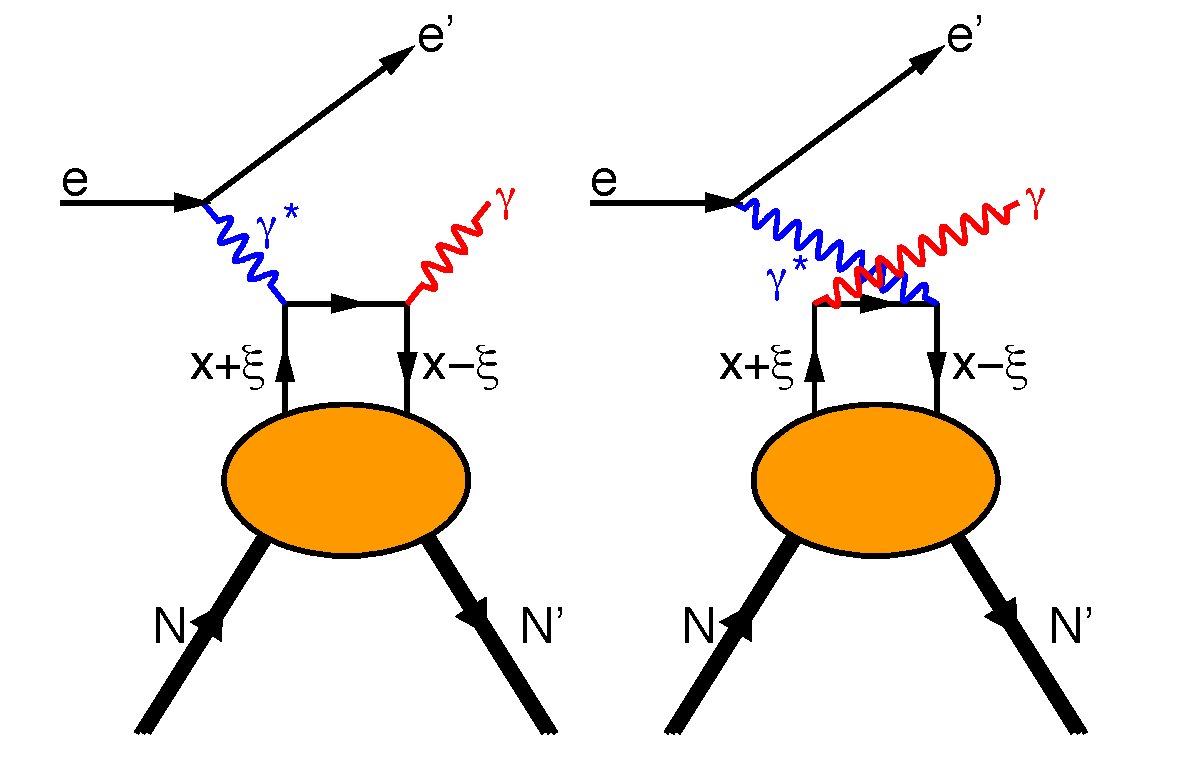
\includegraphics[width=0.45\textwidth]{dvcs_both}}
\subfigure[Bethe-Heitler]{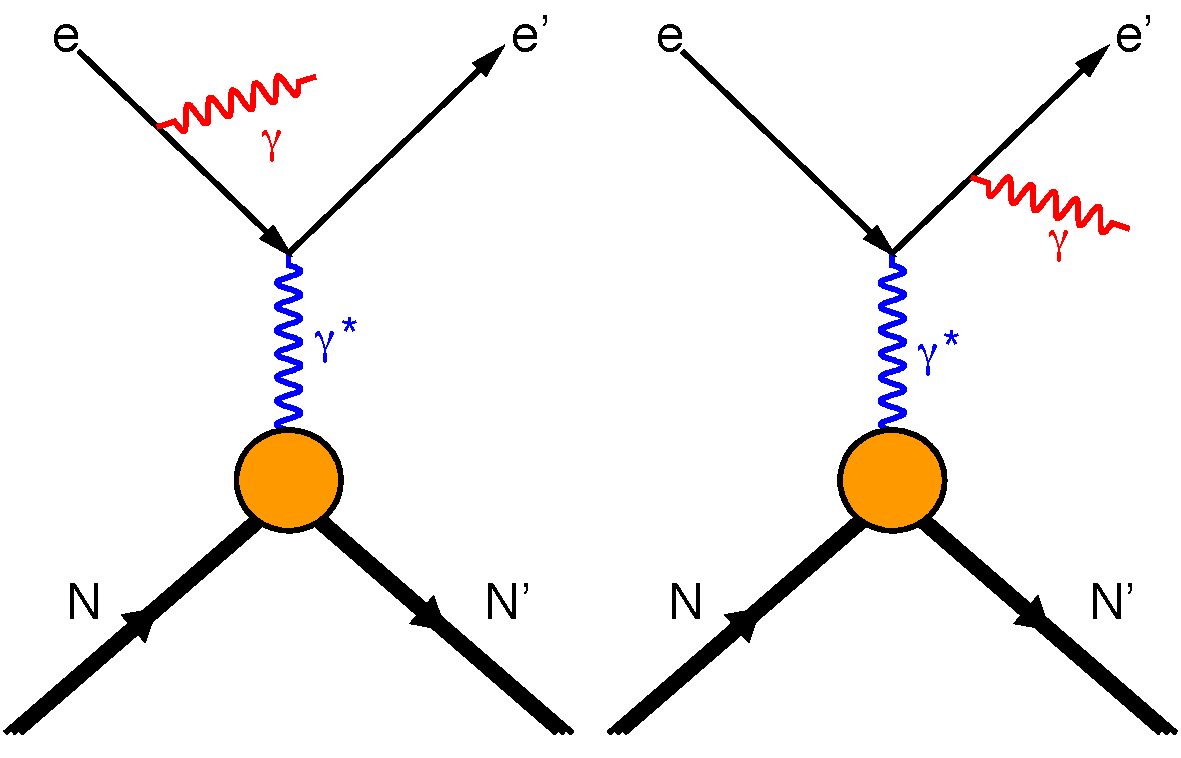
\includegraphics[width=0.45\textwidth]{bh_both}}
\caption[DVCS and Bethe Heitler hand bag diagram.]{(a): The \red{leading} DVCS process in which an electron/positron ($e$) interacts with a quark in the nucleon
($N$) via a virtual photon ($\gamma^\ast$). The quark is found in the
nucleon with longitudinal momentum fraction $x+\xi$ and emits a real
photon ($\gamma$). The quark is absorbed by the nucleon with
longitudinal momentum fraction $x-\xi$. (b): The \red{leading} Bethe-Heitler process, i.e. the emission of a real photon from the scattering or
scattered lepton. It has the same initial and final states as DVCS.}
\label{spin}
\end{center}
\end{figure}


Exclusive leptoproduction of real photons
($e\,N\,\rightarrow\,e'\,N'\,\gamma$) arises from
two experimentally indistinguishable processes: the Deeply Virtual Compton Scattering (DVCS) process,
which is the emission of a real photon by the struck quark from the nucleon, and the Bethe--Heitler (BH) process, which is elastic lepton-\red{nucleon} scattering with the
emission of a Bremsstrahlung photon by the lepton. \red{The leading terms in these processes are shown in figure~\ref{spin}.}
The BH process is calculable in the QED framework; this process is
dominant at the kinematic conditions of the H{\sc ermes} experiment, but the
scattering amplitudes of the two processes interfere and the large BH amplitude
amplifies the contribution of the DVCS amplitude to the interference term. 
It is through the study of this interference term at H{\sc ermes} that
useful information for the constraint of certain GPDs can be obtained \cite{Bel02b}.

The four-fold differential cross section for the \red{exclusive} leptoproduction of real photons
from an unpolarised target can be written as \cite{Bel02b}
\begin{center}
\begin{equation}
\frac{\textrm{d}^4\sigma}{\textrm{d}x_{\textrm{B}}\textrm{d}Q^{2}\textrm{d}
|t|\textrm{d}\phi} =
\frac{x_{\textrm{B}}e^{6}}{32(2\pi)^{4} Q^{4}\sqrt{1+\epsilon^{2}}}
|\tau|^{2},
\end{equation}
\end{center}
where $e$ is the elementary
charge, $\epsilon=2x_\textrm{B}\frac{M}{Q}$ with $M$
the \red{target} mass, and $\phi$ is the
azimuthal angle between the scattering and production planes \cite{Tre04}.
The {square of the} scattering amplitude $|\tau|^2$ can be written as
\begin{center}
\begin{equation}
|\tau|^{2} = |\tau_{\textrm{BH}}|^{2} +
|\tau_{\textrm{DVCS}}|^{2} + \textrm{I},
\end{equation}
\end{center}
with contributions from the \textrm{BH} process ($\tau_{\textrm{\textrm{BH}}}$),
the DVCS process
($\tau_{\textrm{DVCS}}$) and their interference term (I). These
contributions can be written as
\begin{eqnarray}
 |\tau_{\textrm{BH}}|^{2} &=&
 \frac{K_{\textrm{BH}}}{\mathcal{P}_{1}(\phi)\mathcal{P}_{2}(\phi)} \left(c_{0,\textrm{unp}}^{\textrm{BH}} + \sum_{n=1}^2
  c_{n,\textrm{unp}}^{\textrm{BH}}\cos(n\phi)\right), \label{e:tbh}\\
|\tau_{\textrm{DVCS}}|^{2} &=&
K_{\textrm{DVCS}}\left(c_{0,\textrm{unp}}^{\textrm{DVCS}} +
\sum_{n=1}^2
c_{n,\textrm{unp}}^{\textrm{DVCS}}\cos(n\phi) + \lambda
s_{1,\textrm{unp}}^{\textrm{DVCS}}\sin\phi\right)\,\textrm{and}
\label{e:tdvcs}\\
 \textrm{I} &=& \frac{- e_\ell
K_{\textrm{I}}}{\mathcal{P}_{1}(\phi)\mathcal{P}_{2}(\phi)}\left(c_{0,\textrm{unp}}^{\textrm{
I}}+
\sum_{n=1}^3 c_{n,\textrm{unp}}^{\textrm{I}}\cos(n\phi) + \lambda \sum_{n=1}^2
s_{n,\textrm{unp}}^{\textrm{I}}\sin(n\phi)\right),\label{e:ti}
\end{eqnarray}
where $\mathcal{P}_1(\phi)$ and $\mathcal{P}_2(\phi)$ are the lepton propagators
of the BH process, $\lambda$ is the
helicity of the lepton beam and $e_\ell$ is the unit charge of
  the lepton.  The
quantities $K_{\textrm{BH}}=1/(x_\textrm{B}^2t(1+\epsilon^2)^2)$,
$K_{\textrm{DVCS}}=1/Q^2$
and $K_{\textrm{I}}=1/(x_{\textrm{B}}yt)$ are kinematic factors, where
$y$ is the fraction of the beam energy carried by the virtual photon in
the target rest frame. A full
explanation of the Fourier coefficients [$c_{n,\textrm{unp}}^V,s_{n,\textrm{unp}}^W$]
($V\in[\textrm{BH,DVCS},\textrm{I}]$ and $W\in[\textrm{DVCS},\textrm{I}]$) can be found in ref.~\cite{Bel02b}.
 
Two sets of asymmetries measured at H{\sc
ermes} with an unpolarised \red{Hydrogen} target and a polarised electron or positron
beam are considered here:
beam-helicity asymmetries and beam-charge asymmetries. This paper,
like ref.~\cite{Air09}, presents results \red{related to} the following asymmetries:
\begin{align}
\hspace{0.5cm}\mathcal{A}^{\textrm{I}}_{\textrm{LU}}(\phi) &\equiv
\frac{(\textrm{d}\sigma(\phi)^{+\rightarrow} -
\textrm{d}\sigma(\phi)^{+\leftarrow}) -
(\textrm{d}\sigma(\phi)^{-\rightarrow}
- \textrm{d}\sigma(\phi)^{-\leftarrow})}{(\textrm{d}\sigma(\phi)^{+\rightarrow}
+
\textrm{d}\sigma(\phi)^{+\leftarrow}) +
(\textrm{d}\sigma(\phi)^{-\rightarrow}
+ \textrm{d}\sigma(\phi)^{-\leftarrow})}&  \nonumber \\
&=\dfrac{-\dfrac{K_{\textrm{I}}}{\mathcal{P}_{1}(\phi)\mathcal{P}_{2}(\phi)}
\displaystyle\sum_{n=1}^2
s_{n}^{\textrm{I}}\sin(n\phi)}{\dfrac{K_{\textrm{BH}}}{\mathcal{P}_{1}
(\phi)\mathcal{P}_{
2}(\phi)}
\displaystyle\sum_{n=0}^2
c_{n}^{\textrm{BH}}\cos(n\phi) + 
K_{\textrm{DVCS}}\displaystyle\sum_{n=0}^2 c_{n}^{\textrm{DVCS}}\cos(n\phi)},& 
\label{e:alui}
\end{align}

\begin{align}
\mathcal{A}^{\textrm{DVCS}}_{\textrm{LU}}(\phi) &\equiv
\frac{(\textrm{d}\sigma(\phi)^{+\rightarrow} +
\textrm{d}\sigma(\phi)^{-\rightarrow}) -
(\textrm{d}\sigma(\phi)^{+\leftarrow} + 
\textrm{d}\sigma(\phi)^{-\leftarrow})}
{(\textrm{d}\sigma(\phi)^{+\rightarrow} +
\textrm{d}\sigma(\phi)^{-\rightarrow}) +
(\textrm{d}\sigma(\phi)^{+\leftarrow}
+ \textrm{d}\sigma(\phi)^{-\leftarrow})}& \nonumber \\[0.4cm]
%\\ \nonumber
&=\dfrac{ K_{\textrm{DVCS}} s_{1}^{\textrm{DVCS}}\sin\phi}{\dfrac{K_{\textrm{BH}}}{\mathcal{P}_{1}
(\phi)\mathcal{P}_{2}(\phi)}
\displaystyle\sum_{n=0}^2
c_{n}^{\textrm{BH}}\cos(n\phi) + 
K_{\textrm{DVCS}}\displaystyle\sum_{n=0}^2
c_{n}^{\textrm{DVCS}}\cos(n\phi)} \textrm{\, and}&
\label{e:aludvcs}
\end{align}

\begin{align}
\hspace{0.5cm}\mathcal{A}_{\textrm{C}}(\phi) &\equiv  
\frac{(\textrm{d}\sigma(\phi)^{+\rightarrow} +
\textrm{d}\sigma(\phi)^{+\leftarrow}) -
(\textrm{d}\sigma(\phi)^{-\rightarrow}
+ \textrm{d}\sigma(\phi)^{-\leftarrow})}{(\textrm{d}\sigma(\phi)^{+\rightarrow}
+
\textrm{d}\sigma(\phi)^{+\leftarrow}) +
(\textrm{d}\sigma(\phi)^{-\rightarrow}
+ \textrm{d}\sigma(\phi)^{-\leftarrow})}&    \nonumber \\
&=\dfrac{{-\dfrac{K_{\textrm{I}}}{\mathcal{P}_{1}(\phi)\mathcal{P}_{2}(\phi)}
\displaystyle\sum_{n=0}^3
c_{n}^{\textrm{I}}\cos(n\phi)}}{\dfrac{K_{\textrm{BH}}}{\mathcal{P}_{1}
(\phi)\mathcal{P}_
{2}(\phi)}
\displaystyle\sum_{n=0}^2
c_{n}^{\textrm{BH}}\cos(n\phi) + 
K_{\textrm{DVCS}}\displaystyle\sum_{n=0}^2 c_{n}^{\textrm{DVCS}}\cos(n\phi)} ,&
\label{e:ac}
\end{align}
where $\textrm{d}\sigma(\phi)^+$ ($\textrm{d}\sigma(\phi)^-$) refers to
cross sections with positive (negative) beam charge and
$\textrm{d}\sigma(\phi)^\rightarrow$ ($\textrm{d}\sigma(\phi)^\leftarrow$) refer\red{s}
to cross sections taken with beam spin parallel (anti-parallel) to the
beam momentum.

\red{The $s_{n,\textrm{unp}}^{W}$ and $c_{n,\textrm{unp}}^{\textrm{I}}$ Fourier
coefficients depend on ``$\mathcal{C}$-functions'' \cite{{Bel02b}}, each of which is a
combination of complex Compton Form Factors (CFFs). A CFF is a
convolution of a GPD with a hard scattering kernel. Contributions of
GPDs to the cross section may be relatively suppressed by powers of
$1/Q$, the origin of which may be kinematic in nature or due to the
twist-level of the GPD. Leading twist is twist-2. Typically, the
contribution of a twist-$n$ GPD, and hence the corresponding CFF, is
suppressed by $\mathcal{O}(1/Q^{n-2})$. 

\red{T}he leading-twist Fourier coefficients are $s_{1,\textrm{unp}}^{\textrm{I}}$ and $c_{1,\textrm{unp}}^{\textrm{I}}$. Both of these Fourier coefficients have a dominant contribution from the $\mathcal{C}_{\textrm{unp}}^{\textrm{I}}$-function:
\begin{eqnarray}
s_{1,\textrm{unp}}^{\textrm{I}} \approx&\,\,\,\,8\lambda ky(2-y)\mathfrak{Im}\mathcal{C}_{\textrm{unp}}^{\textrm{I}}\quad\textrm{and}&\label{eq:s1}
\\
 c_{1,\textrm{unp}}^{\textrm{I}} \approx&8k(2- 2y + y^{2})\mathfrak{Re}\mathcal{C}_{\textrm{unp}}^{\textrm{I}}\,,&\label{eq:c1}
\end{eqnarray}
where the definition of the kinematic factor $k$ is found
  in ref.\cite{Bel02b}. The $\mathcal{C}_{\textrm{unp}}^{\textrm{I}}$-function can be
written
\cite{Bel02b} 
\begin{equation}
 \mathcal{C}_{\textrm{unp}}^{\textrm{I}} = F_{1}\mathcal{H} + \frac{x_{\textrm{B}}}{2-x_{\textrm{B}}}(F_{1}+F_{2})\widetilde{\mathcal{H}} -\frac{t}{4M^{2}}F_{2}\mathcal{E},
\label{Eq_cunp}
\end{equation}
where $F_{1}$ and $F_{2}$ are respectively the Dirac and Pauli form
factors of the nucleon and $\mathcal{H}$, $\widetilde{\mathcal{H}}$ and
$\mathcal{E}$ are CFFs that relate respectively to the GPDs $H$,
$\widetilde{H}$ and $E$.  At H{\sc ermes} kinematic
conditions (where $x_{\textrm{B}}$ and $\frac{-t}{4M^2}$ are of order 0.1), the
contributions of CFFs $\widetilde{\mathcal{H}}$ and $\mathcal{E}$ can be
neglected in eq.~\ref{Eq_cunp} (in first approximation) with respect to $\mathcal{H}$ since they
are kinematically suppressed by an order of magnitude or more.
Hence, the behaviour of
$\mathcal{C}_{\textrm{unp}}^{\textrm{I}}$ is determined by CFF $\mathcal{H}$
and therefore GPD $H$ can be constrained through
measurements of the $\sin\phi$ and $\cos\phi$ terms of the $\mathcal{A}^{\textrm{I}}_{\textrm{LU}}(\phi)$ and $\mathcal{A}_{\textrm{C}}(\phi)$ asymmetries respectively.}

Compared to the analysis in ref.~\cite{Air09}, the analysis presented here additionally includes a larger,
independent data set taken during the years 2006 and 2007 after the
experiment was upgraded in the target region. The work covered
  in this publication combines the data taken in 1996-2005 with this
  new data set to produce the largest DVCS data set that will be published by H{\sc ermes}.
The results in this paper make use of the same missing-mass technique for event selection as was used in ref.~\cite{Air09}.

\section{Experiment and Data Selection}
The data were collected in 2006 and 2007 with the H{\sc ermes}
spectrometer \cite{Ack98} using the longitudinally polarised 27.6\,GeV
electron and positron beams incident upon an unpolarised hydrogen gas
target internal to the HERA lepton storage ring at DESY. The integrated
luminosities of the electron and positron data samples respectively are
approximately 246\,pb$^{-1}$ and 1460\,pb$^{-1}$, with average beam polarisations of 30.3\,\% and 39.2\% \cite{Ben01}. The procedure used to select events is similar to that used in Ref.~\cite{Air09}.
A brief summary of this procedure is outlined in the following; consult
Refs.~\cite{Zei09,Bur10} for more details. An event
was selected as having exactly one photon and one lepton
track detected within the acceptance of the spectrometer.

The event selection is subject to the kinematic constraints 1\,GeV$^{2}$ $<$
Q$^{2}$ $<$ 10\,GeV$^{2}$, 0.03 $<$ $x_{\textrm{B}}$ $<$ 0.35, $W^{2}$ $>$
9\,GeV$^{2}$ and $\nu$ $<$ 22\,GeV, where $W$ is the invariant mass of the
$\gamma^{*}p$ system and $\nu$ is the energy of the virtual photon in the target
rest frame. The polar angle between the virtual and real photons was required to
be within the limits 5 mrad $<$
$\theta_{\gamma^{*}\gamma}$ $<$ 45 mrad. 

An event sample was selected using a missing-mass technique requiring that the squared missing-mass $M_{\textrm{X}}^{2}=(q+p-q')^{2}$ of the $ep \rightarrow e\gamma \textrm{X}$ measurement corresponded to the square of the proton mass within the limits of the energy resolution of the calorimeter. Here, $q$ is the four-momentum of the virtual photon, $p$ is the \blue{initial} four-momentum of the target proton and $q'$ is the four\blue{-}momentum of the produced photon. The ``exclusive region'' was defined as ($-1.5$\,GeV)$^{2} < M_{\textrm{X}}^{2}$ $<$ (1.7\,GeV)$^{2}$, as in Ref.~\cite{Air09}. This exclusive region was shifted by up to 0.17\,GeV$^{2}$ to reflect observed differences in the distributions of the electron and positron data samples and to account for the time dependence of the missing-mass distributions observed in the 2007 data set \cite{Bur10}. 

\section{Experimental Extraction of Asymmetry Amplitudes}

The expectation value of the experimental yield $N$ is parameterised as
\begin{equation}
 \langle N(e_{\ell},P_{\ell},\phi)\rangle =
\mathcal{L}(e_{\ell},P_{\ell})\eta(e_{\ell},\phi)\textrm{d}\sigma_{UU}
(\phi)\times
[1+P_{\ell}\mathcal{A}_{\textrm{LU}}^{\textrm{DVCS}}(\phi)+e_{\ell}P_{\ell}
\mathcal{A}_{\textrm{LU}}^{\textrm{I}}(\phi)+e_{\ell}\mathcal{A}_{\textrm{C}}
(\phi)],
\end{equation}
where $\mathcal{L}$ is the integrated luminosity, $\eta$ the detection
efficiency and d$\sigma_{UU}$ denotes the
cross section for an unpolarised target integrated over both beam charges and
beam helicities. The asymmetries $\mathcal{A}_{\textrm{LU}}^{\textrm{I}}(\phi)$,
$\mathcal{A}_{\textrm{LU}}^{\textrm{DVCS}}(\phi)$ and
$\mathcal{A}_{\textrm{C}}(\phi)$ are expanded in
$\phi$ as
\begin{equation}
\mathcal{A}_{\textrm{LU}}^{\textrm{I}}(\phi) \simeq \sum^{2}_{n=1}
A_{\textrm{LU,I}}^{\sin(n\phi)}\sin(n\phi) 
+ \sum^{1}_{n=0} A_{\textrm{LU,I}}^{\cos(n\phi)}\cos(n\phi),
\label{alui_asym}
\end{equation}
\begin{equation}
 \mathcal{A}_{\textrm{LU}}^{\textrm{DVCS}}(\phi) \simeq \sum^{2}_{n=1}
A_{\textrm{LU,DVCS}}^{\sin(n\phi)}\sin(n\phi) 
+ \sum^{1}_{n=0} A_{\textrm{LU,DVCS}}^{\cos(n\phi)}\cos(n\phi),
\label{aludvcs_asym}
\end{equation}
\begin{equation}
\mathcal{A}_{\textrm{C}}(\phi) \simeq \sum^{3}_{n=0}
A_{\textrm{C}}^{\cos(n\phi)}\cos(n\phi) 
+ A_{\textrm{C}}^{\sin\phi}\sin\phi,
\label{ac_asym}
\end{equation}
where the approximation is due to the truncation of the infinite Fourier series
caused by the azimuthal dependencies in the denominators from
Eqs.~\ref{e:alui}-\ref{e:ac}. Only the $\sin(n\phi)$ terms of the
$\mathcal{A}_{\textrm{LU}}$ asymmetries and the $\cos(n\phi)$ terms of the
$\mathcal{A}_{\textrm{C}}$ asymmetry are physically motivated. The other terms
are included as both a consistency check for extraneous harmonics caused
by the denominators in Eqs.~\ref{e:alui}-\ref{e:ac} and as a test of the
normalisation of the fit. These terms are expected to be small.

A maximum-likelihood fitting technique \cite{Bar90} was used to
extract the asymmetry amplitudes in each kinematic bin of $-t$, $x_{\textrm{B}}$ and $Q^{2}$.
This method, described in Ref.~\cite{Air08}, fits the expected
azimuthal distribution function to the data without introducing binning effects in $\phi$.
Weights are introduced per event in the fitting procedure to account for
luminosity imbalances with respect to the beam charge and polarisation.

The asymmetry amplitudes $A_{\textrm{LU,I/DVCS}}^{\sin(n\phi)}$ and
$A_{\textrm{C}}^{\cos(n\phi)}$ relate respectively to the Fourier
coefficients $s_{n}^{W}$ and $c_{n}^{V}$ from the interference and DVCS terms in Eqs.~\ref{e:alui}-\ref{e:ac}. The asymmetry amplitudes may also be affected by the lepton \blue{propagators} and the other $\phi$-dependent terms in the denominators in Eqs.~\ref{e:alui}-\ref{e:ac}. The  $s_{n}^{W}$ and $c_{n}^{V}$ Fourier coefficients depend on ``$\mathcal{C}$-functions'', each of which is a combination of complex Compton Form Factors. A CFF is a convolution of a GPD with a hard scattering kernel. Contributions of GPDs to the cross section may be relatively suppressed by powers of $1/Q$, the origin of which may be kinematic in nature or due to the twist level of the GPD. The access from each asymmetry amplitude to a GPD is called twist-$n$ depending upon the part of the twist-decomposed cross-section in which the amplitude appears. Leading twist is twist-2. Typically, the contribution of a twist-$n$ GPD, and hence the corresponding CFF, is suppressed by $\mathcal{O}(1/Q^{n-2})$. Table~\ref{tab_amplitudes} presents the asymmetry amplitudes extracted in this analysis and the related Fourier coefficients, dominant $\mathcal{C}$-function, twist-level and levels of suppression.

At H{\sc ermes} kinematic conditions, the leading-twist beam-helicity asymmetry amplitude is $A_{\textrm{LU,I}}^{\sin\phi}$ and the leading beam-charge asymmetry amplitude is $A^{\cos\phi}_{\textrm{C}}$. These asymmetry amplitudes for an unpolarised target are sensitive respectively to Fourier coefficients $s_{1,\textrm{unp}}^{\textrm{I}}$ and $c_{1,\textrm{unp}}^{\textrm{I}}$. Both of these Fourier coefficients have a dominant contribution from the $\mathcal{C}_{\textrm{unp}}^{\textrm{I}}$-function:
\begin{center}
\begin{equation}
 s_{1,\textrm{unp}}^{\textrm{I}} \approx 8\lambda ky(2-y)\mathfrak{Im}\mathcal{C}_{\textrm{unp}}^{\textrm{I}},
\label{eq:s1}
\end{equation}
\end{center}
\begin{center}
\begin{equation}
 c_{1,\textrm{unp}}^{\textrm{I}} \approx 8k(2- 2y + y^{2})\mathfrak{Re}\mathcal{C}_{\textrm{unp}}^{\textrm{I}},
\label{eq:c1}
\end{equation}
\end{center}
where the kinematic factor $k \propto \sqrt{-t}/Q$ originates from the BH
propagators. The $\mathcal{C}_{\textrm{unp}}^{\textrm{I}}$-function can be
written
\cite{Bel02b} 
\begin{equation}
 \mathcal{C}_{\textrm{unp}}^{\textrm{I}} = F_{1}\mathcal{H} + \frac{x_{\textrm{B}}}{2-x_{\textrm{B}}}(F_{1}+F_{2})\widetilde{\mathcal{H}} -\frac{t}{4M^{2}}F_{2}\mathcal{E},
\label{Eq_cunp}
\end{equation}
where $F_{1}$ and $F_{2}$ are respectively the Dirac and Pauli form
factors of the nucleon and $\mathcal{H}$, $\widetilde{\mathcal{H}}$ and
$\mathcal{E}$ are CFFs that relate respectively to the GPDs $H$,
$\widetilde{H}$ and $E$.  At H{\sc ermes} kinematic
conditions (where $x_{\textrm{B}}$ and $\frac{t}{4M^2}$ are of order 0.1), to first approximation the
contributions of CFFs $\widetilde{\mathcal{H}}$ and $\mathcal{E}$ can be
neglected in Eq.~\ref{Eq_cunp} with respect to $\mathcal{H}$ since they
are kinematically suppressed by an order of magnitude or more.
Hence, in this approximation, the behaviour of
$\mathcal{C}_{\textrm{unp}}^{\textrm{I}}$ is determined by CFF $\mathcal{H}$
and therefore GPD $H$. Using this dependence, $H$ can be constrained through
measurements of $A_{\textrm{LU,I}}^{\sin\phi}$ and $A^{\cos\phi}_{\textrm{C}}$.
The asymmetry amplitudes $A_{\textrm{LU},\textrm{I}}^{\sin(2\phi)}$,
$A^{\cos(0\phi)}_{\textrm{C}}$ and $A^{\cos(2\phi)}_{\textrm{C}}$ also depend
upon this $\mathcal{C}$-function. However, the $A^{\cos(0\phi)}_{\textrm{C}}$ amplitude is kinematically suppressed compared to the $A^{\cos\phi}_{\textrm{C}}$ amplitude, and the  $A_{\textrm{LU,I}}^{\sin(2\phi)}$ and $A^{\cos(2\phi)}_{\textrm{C}}$ amplitudes enter the cross section at a higher
twist level (see Table~\ref{tab_amplitudes}).

The DVCS asymmetry amplitude $A^{\sin\phi}_{\textrm{LU,DVCS}}$ has a
contribution from the $\mathcal{C}_{\textrm{unp}}^{\textrm{DVCS}}$ function,
which is bilinear in CFFs. \blue{However, this amplitude is inherently small at HERMES kinematic conditions due to the size of the $s_{1}^{\textrm{DVCS}}$ Fourier coefficient compared to the $s_{1}^{\textrm{I}}$ coefficient.} As a result of
the more complicated dependence on the CFFs and this suppression, it
will be more difficult to extract useful information for the constraint of GPDs
from the measurement of $A^{\sin\phi}_{\textrm{LU,DVCS}}$ than from the
kinematically-unsuppressed leading-twist amplitudes.

The $A^{\cos(3\phi)}_{\textrm{C}}$ amplitude depends on the
$c_{3,\textrm{unp}}^{\textrm{I}}$ Fourier coefficient and hence the
$\mathcal{C}_{\textrm{T,unp}}^{\textrm{I}}$ function. This
$\mathcal{C}$-function receives contributions from both the BH and DVCS
processes and therefore depends on $F_{1}$, $F_{2}$ and CFFs. Although the CFFs
in this function are of leading twist, they relate to gluon helicity-flip GPDs and are thus suppressed by $\alpha_{\textrm{S}}/\pi$.
\begin{table}[H]
\begin{center}
\resizebox{16cm}{!} {
 \begin{tabular}{|c|c|c|c|c|}
\hline
Asymmetry Amplitude & Fourier Coefficient& Dominant CFF Dependence & Twist Level  & Relative Suppression \\
\hline
\hline
$A_{\textrm{LU,I}}^{\sin\phi}$ & $s_{1,\textrm{unp}}^{\textrm{I}}$  &
$\mathfrak{Im}\mathcal{C}_{\textrm{unp}}^{\textrm{I}}$
&  2 & --\\
\hline
$A_{\textrm{LU,I}}^{\sin(2\phi)}$ & $s_{2,\textrm{unp}}^{\textrm{I}}$ 
&
$\mathfrak{Im}\mathcal{C}_{\textrm{unp}}^{\textrm{I}}$
&  3 & $1/Q$\\
\hline
\hline
$A_{\textrm{LU,DVCS}}^{\sin\phi}$ & $s_{1, \textrm{unp}}^{\textrm{DVCS}}$ &
$\mathfrak{Im}\mathcal{C}_{\textrm{unp}}^{\textrm{DVCS}}$ &  3 & $1/Q$ \\
\hline
\hline
$A_{\textrm{C}}^{\cos(0\phi)}$ & $c_{0,\textrm{unp}}^{\textrm{I}}$  &
$\mathfrak{Re}\mathcal{C}_{\textrm{unp}}^{\textrm{I}}$ & 2& --
\\
\hline
$A_{\textrm{C}}^{\cos\phi}$ & $c_{1,\textrm{unp}}^{\textrm{I}}$  &
$\mathfrak{Re}\mathcal{C}_{\textrm{unp}}^{\textrm{I}}$ & 2 & --
\\
\hline
$A_{\textrm{C}}^{\cos(2\phi)}$ & $c_{2,\textrm{unp}}^{\textrm{I}}$ &
$\mathfrak{Re}\mathcal{C}_{\textrm{unp}}^{\textrm{I}}$ & 3 & $1/Q$ \\
\hline
$A_{\textrm{C}}^{\cos(3\phi)}$ & $c_{3,\textrm{unp}}^{\textrm{I}}$ &
$\mathfrak{Re}\mathcal{C}_{\textrm{T,unp}}^{\textrm{I}}$ &  2 & $\alpha_{\textrm{S}}/\pi$ \\
\hline
 \end{tabular}
}
\caption{Asymmetry amplitudes that can
be extracted from the available data set, the related Fourier coefficients,
 the $\mathcal{C}$-functions, the twist level and the suppression at H{\sc ermes} kinematic conditions~\cite{Bel02b}.}
\label{tab_amplitudes}
\end{center}
\end{table}
 

\section{Background Corrections and Systematic Uncertainties}
The extracted asymmetry amplitudes are subject to systematic uncertainties that
result from a combination of background processes, 
shifts in the missing-mass distributions and various detector and binning
effects determined as in Refs.~\cite{Air08,Air09}. Contributions to the uncertainties on the amplitude measurements arise from background in the data from neutral meson production. The procedure is described in detail in Refs.~\cite{Air08,Air09} and the contributions to the uncertainties of the measurements addressed here are given in Table~\ref{table_systematic_contributions_0607} for the amplitudes extracted in a single bin in the H{\sc ermes} kinematic region. 

Another contribution to the systematic uncertainty comes from the relative shift of the
missing-mass distributions. \blue{There are shifts in the distributions for electron and positron data~\cite{Zei09,Bur10}}. \blue{The missing-mass
distribution is also adjusted for each calorimeter calibration period of data
collected in 2007 to account for the observed time dependence.} One
quarter of the difference between the asymmetries extracted using the standard
and shifted missing-mass windows is taken as the corresponding systematic
uncertainty. The beam polarisation measurement has a total uncertainty of 2.8\% and 3.4\% for the 1996-2005 and 2006-2007 data taking periods respectively,
which is present in the beam-helicity amplitudes and is quoted as an
independent scale uncertainty.

The predominant contribution to the systematic uncertainty arises from detector
effects, including the acceptance of the spectrometer, smearing effects due to detector resolution and radiative processes, and
finite bin width in $-t$, $x_{\textrm{B}}$ and $Q^{2}$. In order to quantify
these effects, events were generated using a Monte Carlo simulation of
the spectrometer that included them. An event
generator based on the GPD model described in Ref.~\cite{Guz06} was used for the simulation because it describes the data well and is consistent with Ref.~\cite{Air09}. Asymmetry amplitudes were extracted from these simulated events using the same analysis
procedure used to extract amplitudes from experimental data. In each kinematic
bin, the systematic uncertainty was determined as the difference between the
asymmetry amplitude reconstructed from the simulated data and that
calculated from the same GPD model at the average $-t$, $x_{\textrm{B}}$ and
$Q^{2}$ value for that bin.
The total systematic uncertainty for the 2006-2007 data sample was
determined for each kinematic bin from the uncertainty contributions of the
background corrections, detector effects and missing-mass shift
uncertainties added in quadrature. 
\blue{The 1996-2005 sample also has a systematic uncertainty from misalignment of the spectrometer, 
which has been eliminated for the 2006-2007 data sample.}
These contributions are summarised in Table
\ref{table_systematic_contributions_0607}.

The data sample in the exclusive region contains events involving both
production of real photons in which the proton remains intact and
events involving the excitation of the target proton to a $\Delta^+$
resonant state. \blue{The} recoiling proton is not detected \blue{and
  the calorimeter resolution does not allow} separation of the latter events from rest of the data sample.
No systematic uncertainty is assigned for the contribution from these events; they are treated as part of the signal. A Monte Carlo calculation based on the parameterisation \blue{from} Ref.~\cite{Bra76} is used to estimate the contribution to the event sample from resonant production in each kinematic bin. The results, denoted associated fraction and labelled ``Assoc. fraction'', are shown in the last row of each figure in the results section. The method used to perform \blue{this} estimation is described in detail in
Ref.~\cite{Air08}.

\begin{table}
 \begin{center}
\resizebox{16cm}{!} {
 \begin{tabular}{|c|c|c|c|c|c|c|}
  \hline
 & $A$ $\pm$ $\delta_{stat.}$ $\pm$ $\delta_{syst.}$ & Background & Missing-Mass Shift & Detector Effects & & Total \\
  \hline
  \hline
  $A_{\textrm{LU,I}}^{\sin\phi}$ & -0.209  $\pm$  0.026  $\pm$   0.026 & 0.005 & 0.005 & 0.025 & & 0.026 \\
  \hline
  $A_{\textrm{LU,DVCS}}^{\sin\phi}$ & -0.015  $\pm$  0.026  $\pm$  0.008 & 0.004 & 0.007 & 0.001 & & 0.008 \\
  \hline
  $A_{\textrm{LU,I}}^{\sin(2\phi)}$ & 0.005  $\pm$  0.025  $\pm$   0.005 & 0.005 & 0.001 & 0.002 & & 0.006 \\
  \hline
  \hline
  $A_{\textrm{C}}^{\cos(0\phi)}$ & -0.039 $\pm$  0.004 $\pm$  0.008 & 0.001 & 0.004 & 0.007 & & 0.008 \\
  \hline
  $A_{\textrm{C}}^{\cos\phi}$ & 0.032  $\pm$  0.006 $\pm$   0.003 & 0.002 & 0.001 & 0.002 & & 0.003 \\
  \hline
  $A_{\textrm{C}}^{\cos(2\phi)}$ & -0.007  $\pm$  0.006  $\pm$   0.002 & 0.001 & 0.001 & 0.001 & & 0.002 \\
  \hline
  $A_{\textrm{C}}^{\cos(3\phi)}$ & 0.009  $\pm$   0.006   $\pm$   0.001 & 0.000 & 0.001 & 0.001 & & 0.001 \\
  \hline
 \end{tabular}
}
  \caption{The contributions to the systematic uncertainty due to the
background correction, the time-dependent shifts of the missing-mass
distributions and detector effects for the 2006-2007 data to the total
systematic uncertainty. The total systematic uncertainties, shown in the
right-most column, are the individual contributions added in quadrature.}
  \label{table_systematic_contributions_0607}
\end{center}
\end{table}


\section{Results}
Results for the beam-helicity and beam-charge asymmetry amplitudes extracted separately from previously published 1996-2005 and the new 2006-2007 hydrogen data sets, are presented in Figs. \ref{release_bsa_0607} and \ref{release_bca_0607}. Each of the asymmetry amplitudes is shown extracted in one bin over all kinematic variables (``overall'') and also projected against $-t$, $x_{\textrm{B}}$ and $Q^{2}$. All of the extracted asymmetry amplitudes are subject to a fractional contribution to the event yield from associated production (``Assoc. fraction''), which is shown in the bottom row of each figure. The beam-helicity asymmetry amplitudes are subject to an additional scale uncertainty from the measurement of the beam polarisation, which is stated in the captions of the figures.
\begin{figure}
\begin{center}
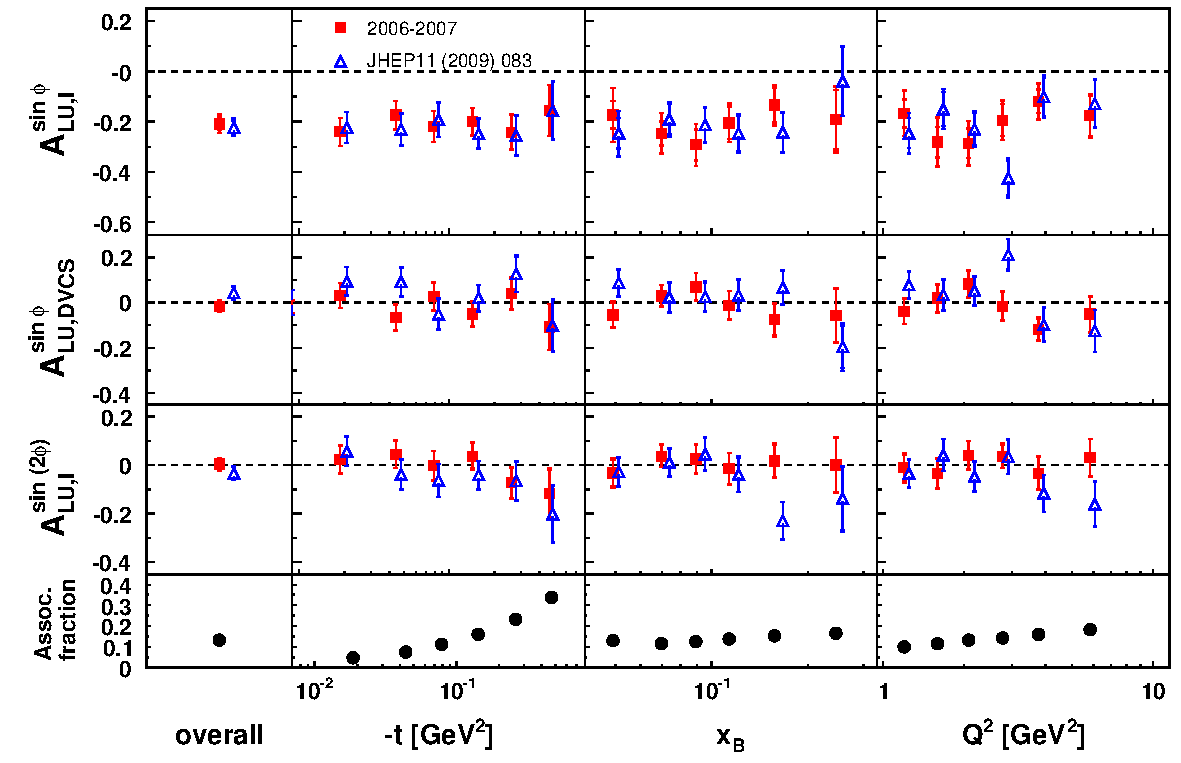
\includegraphics[width=15cm,keepaspectratio]{bsadvcsplots_eml_par13_bin6_release_pic_update_0607_9605}
  \caption{Beam-helicity asymmetry amplitudes extracted separately from
the 1996-2005 (open triangles) and 2006-2007 (filled squares)
hydrogen data. The inner error bars represent the statistical uncertainties, while total error bars denote the statistical and systematic uncertainties added in quadrature.  
An additional 2.8\,\% and 3.4\,\% scale uncertainty for the 1996-2005 and
2006-2007 data respectively is present in the amplitudes due to the imprecision of
the beam polarisation measurement. The simulated fractional contribution from associated production to the yield in each kinematic bin is shown in the bottom row.}
 \label{release_bsa_0607}
\end{center}
 \end{figure}

A statistical test was applied in order to check for possible incompatiability between the asymmetry amplitudes extracted from both data sets. Only the statistical uncertainties were employed in this test. The results show that the two data sets are not incompatible. The $A_{\textrm{LU,I}}$, $A_{\textrm{LU,DVCS}}$ and $A_{\textrm{C}}$ asymmetry amplitudes can therefore be extracted from the complete hydrogen data set recorded during the entire experimental operation of H{\sc ermes}.
\begin{figure}
\begin{center}
 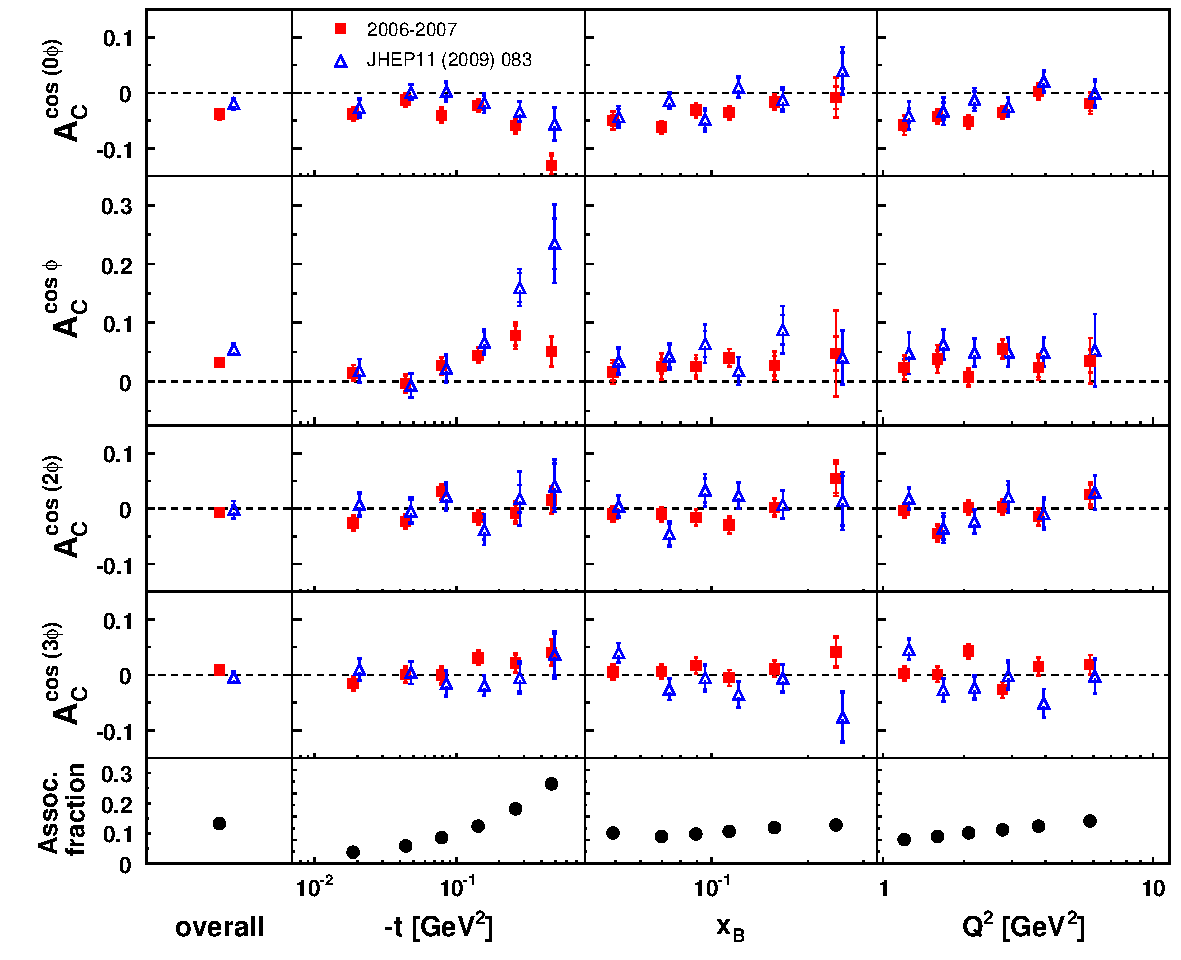
\includegraphics[width=15cm,keepaspectratio]{bcaplots_eml_par13_bin6_release_pic_update_0607_9605_withassoc}
  \caption{Beam-charge asymmetry amplitudes extracted separately from the 1996-2005 (open triangles) and 2006-2007 (filled squares) hydrogen data.
The inner error bars represent the statistical uncertainties, while the total error bars denote the statistical and systematic uncertainties added in quadrature. The simulated fractional contribution from associated production to the yield in each kinematic bin is shown in the bottom row.}
 \label{release_bca_0607}
\end{center}
 \end{figure}

\begin{figure}
 \begin{center}
 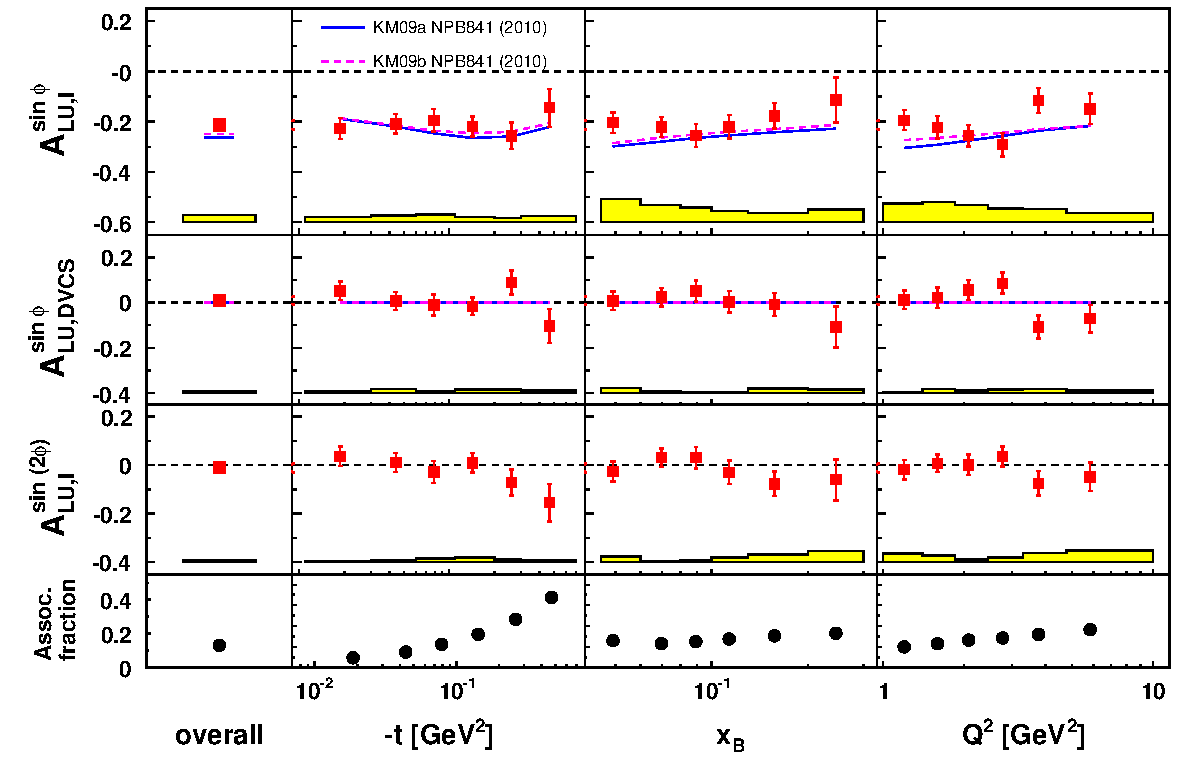
\includegraphics[width=15cm]{bsadvcsplots_eml_par13_bin6_release_all_pic_update}
  \caption{The $A_{\textrm{LU,I}}^{\sin\phi}$, $A_{\textrm{LU,DVCS}}^{\sin\phi}$ and
$A_{\textrm{LU,I}}^{\sin(2\phi)}$ beam-helicity \blue{asymmetry} amplitudes extracted from all the hydrogen data recorded at H{\sc ermes}
from 1996 until 2007. The error bars (bands) represent the statistical
(systematic) uncertainties. \blue{An additional 3.2\,\% scale uncertainty is present in the amplitudes due to the imprecision of
the beam polarisation measurement.} Theoretical calculations from the model described in \cite{Kum09} are shown as solid and dashed lines. See text for details. The simulated fractional contribution from associated production to the yield in each kinematic bin is shown in the bottom row.}
  \label{bsa_xbjrange}
 \end{center}
\end{figure}

\begin{figure}
  \begin{center}
    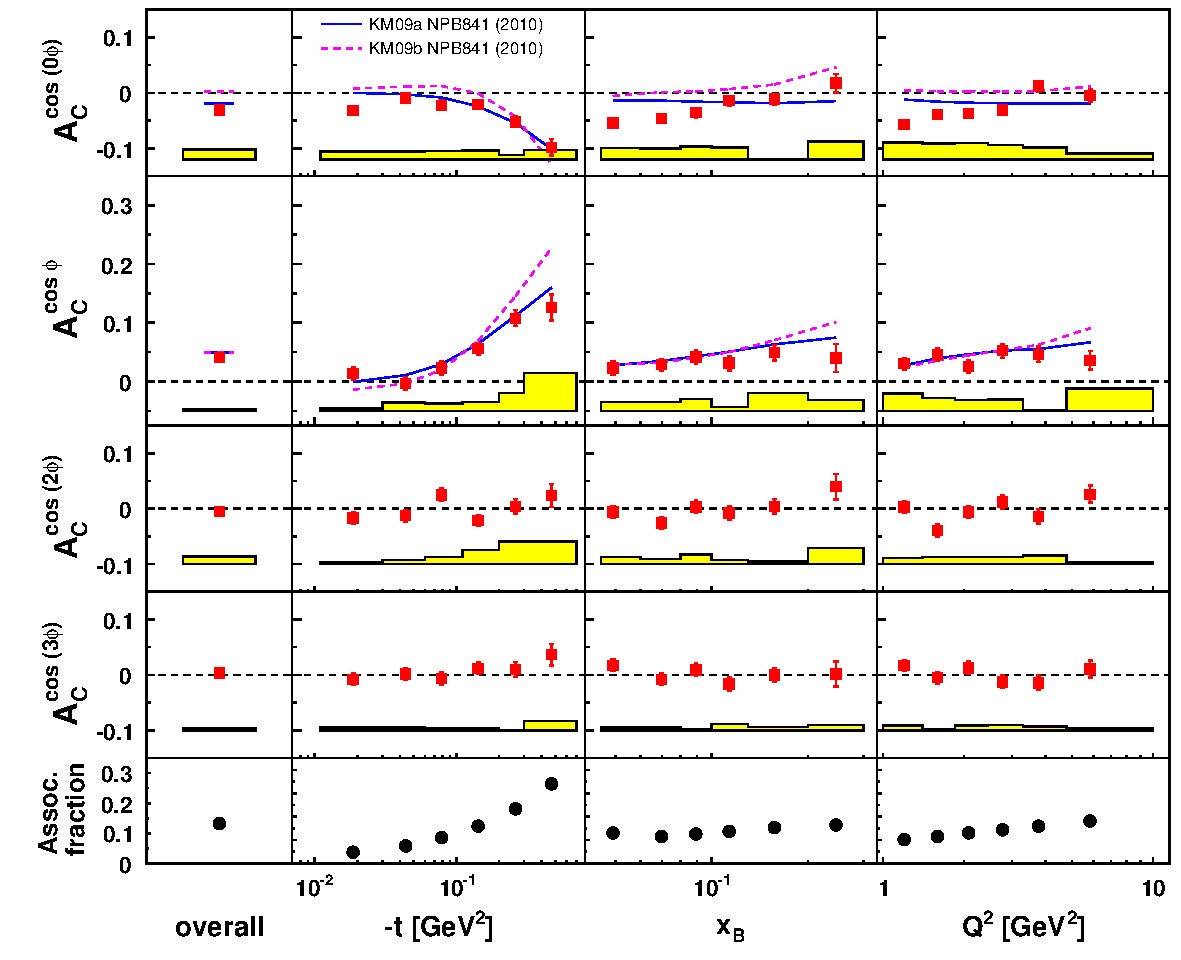
\includegraphics[width=15cm]{bcaplots_eml_par13_bin6_all_release_pic_update_withassoc}
    \caption{The $A_{\textrm{C}}^{\cos(0\phi)}$, $A_{\textrm{C}}^{\cos\phi}$, $A_{\textrm{C}}^{\cos(2\phi)}$ and $A_{\textrm{C}}^{\cos(3\phi)}$ beam-charge \blue{asymmetry} amplitudes extracted from all the hydrogen data recorded at H{\sc ermes} from 1996 until 2007. The error bars (bands) represent the statistical (systematic) uncertainties.  Theoretical calculations from the model described in \cite{Kum09} are shown as solid and dashed lines. See text for details. The simulated fractional contribution from associated production to the yield in each kinematic bin is shown in the bottom row.}
  \label{bca_xbjrange}
 \end{center}
\end{figure}

\begin{figure}
 \begin{center}
 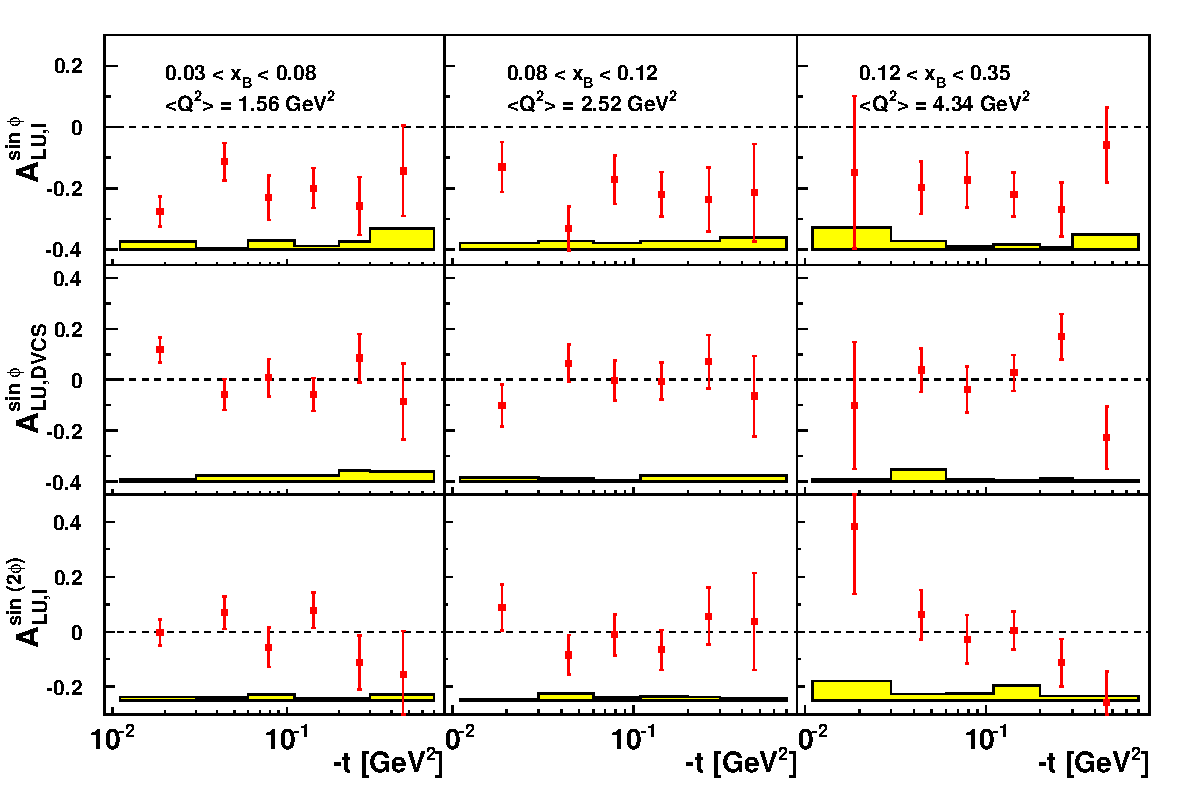
\includegraphics[width=15cm]{bsadvcsplots_tc_xbjrange_eml_par13_bin6_9607_pic_update}
  \caption{\blue{The $A_{\textrm{LU,I}}^{\sin\phi}$, $A_{\textrm{LU,DVCS}}^{\sin\phi}$ and
$A_{\textrm{LU,I}}^{\sin(2\phi)}$ beam-helicity asymmetry amplitudes extracted from all the hydrogen data recorded at H{\sc ermes}
from 1996 until 2007 as a function of $-t$ for three different $x_{\textrm{B}}$ ranges. The error bars (bands) represent the statistical
(systematic) uncertainties. An additional 3.2\,\% scale uncertainty is present in the amplitudes due to the imprecision of
the beam polarisation measurement.}}
  \label{bsa_xbjrange2}
 \end{center}
\end{figure}

\begin{figure}
  \begin{center}
    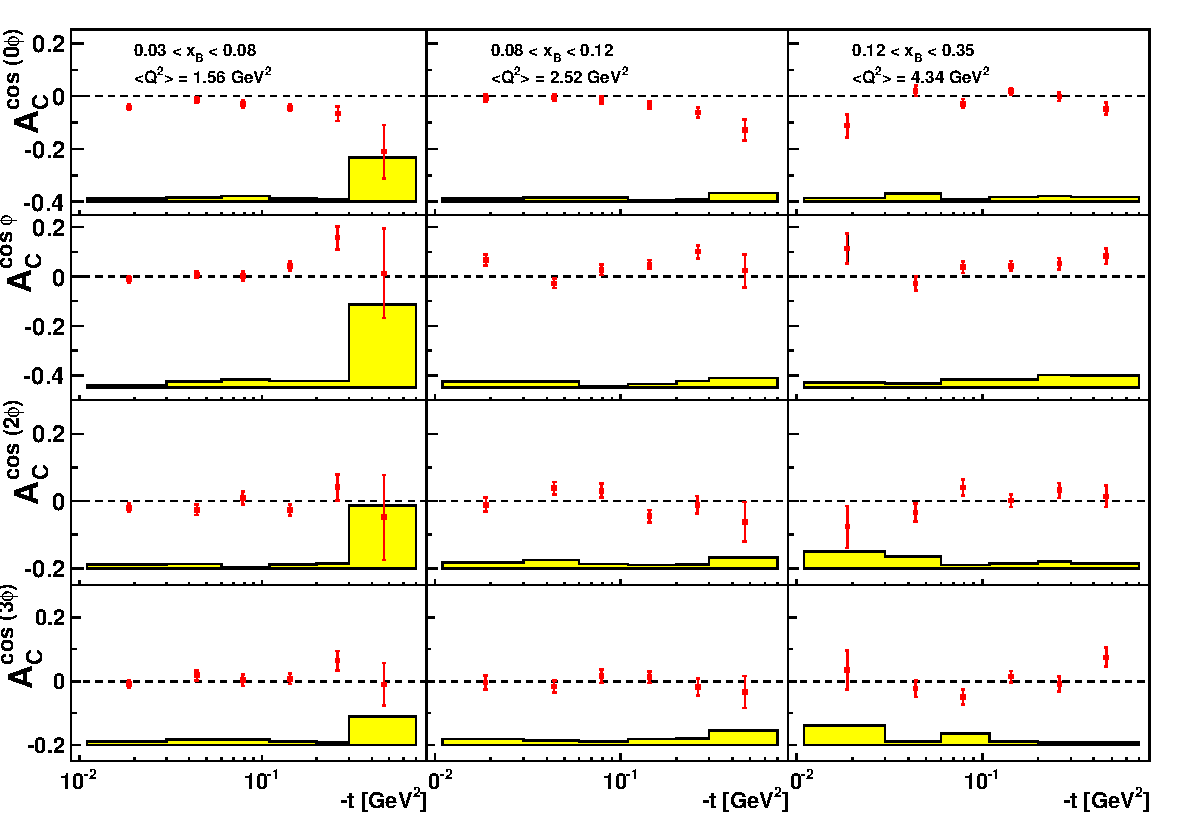
\includegraphics[width=15cm]{bcaplots_tc_xnjrange_eml_par13_bin6_9607_pic}
    \caption{\blue{The $A_{\textrm{C}}^{\cos(0\phi)}$, $A_{\textrm{C}}^{\cos\phi}$, $A_{\textrm{C}}^{\cos(2\phi)}$ and $A_{\textrm{C}}^{\cos(3\phi)}$ beam-charge asymmetry amplitudes extracted from all the hydrogen data recorded at H{\sc ermes} from 1996 until 2007 as a function of $-t$ for three different $x_{\textrm{B}}$ ranges. The error bars (bands) represent the statistical (systematic) uncertainties.}}
  \label{bca_xbjrange2}
 \end{center}
\end{figure}

The results of the beam-helicity and beam-charge asymmetry amplitudes extracted from the complete 1996-2007 hydrogen sample are shown in Figs.~\ref{bsa_xbjrange} and \ref{bca_xbjrange}. The number of analysable events available from the 2006-2007 data set (67815) is approximately three times greater than the number \blue{of} events recorded in the 1996-2005 sample (24817). The  asymmetry amplitudes extracted from the complete 1996-2007 data set are thus weighted towards the 2006-2007 result. \blue{This is not so evident for the beam helicity asymmetry amplitudes} because the beam polarisation was lower in 2006 and 2007.

The first and second harmonics of $\mathcal{A}_{\textrm{LU,I}}$, which are
sensitive to the interference term in the scattering amplitude, are shown in the first and third rows of Fig.~\ref{bsa_xbjrange}. The leading-twist amplitude $A_{\textrm{LU,I}}^{\sin\phi}$ has the largest value of any of the amplitudes when extracted in a single bin from the entire data set. This amplitude has no strong dependence on $-t$, $x_{\textrm{B}}$ or $Q^{2}$, implying a strong dependence at smaller values of $-t$ as the amplitude must diminish \blue{in this $-t$ region} due to the dependence of the amplitude on the factor $k$ from Eq.~\ref{eq:s1}. The $A_{\textrm{LU,I}}^{\sin\phi}$ amplitude is sensitive to the imaginary part of the CFF $\mathcal{H}$ and thereby can constrain GPD $\textit{H}$. The twist-3 $A_{\textrm{LU,I}}^{\sin(2\phi)}$ amplitude \blue{is} compatible with zero, as \blue{is} the twist-3 $A_{\textrm{LU,DVCS}}^{\sin\phi}$ amplitude, which is dependent on the squared DVCS term. The $A_{\textrm{LU,DVCS}}^{\sin\phi}$ amplitudes are shown in the second row of Fig.~\ref{bsa_xbjrange}. Neither the $A_{\textrm{LU,DVCS}}^{\sin\phi}$ nor the $A_{\textrm{LU,I}}^{\sin(2\phi)}$ amplitude show any clear dependence on $-t$, $x_{\textrm{B}}$ or $Q^{2}$. The systematic error bands of the asymmetry amplitudes extracted from the combined data set were determined using Monte Carlo simulations that reflect the equipment used in the various stages of the H{\sc ermes} experiment. 

The $A_{\textrm{C}}^{\cos(n\phi)}$ amplitudes are shown in Fig.~\ref{bca_xbjrange}. The leading-twist $A_{\textrm{C}}^{\cos(0\phi)}$ and $A_{\textrm{C}}^{\cos\phi}$ amplitudes are both non-zero. There is a relationship between $A_{\textrm{C}}^{\cos(0\phi)}$ and $A_{\textrm{C}}^{\cos\phi}$ as the Fourier coefficient $c^{\textrm{I}}_{0,\textrm{UNP}}$ is inversely proportional to $c^{\textrm{I}}_{1,\textrm{UNP}}$ via the kinematic factor $k$ \blue{from} Eq.~\ref{eq:c1}. These amplitudes diverge with opposite sign from zero at increasing values of $-t$ but they
have no discernible dependence on $x_{\textrm{B}}$ and $Q^{2}$. The $A_{\textrm{C}}^{\cos(2\phi)}$ and $A_{\textrm{C}}^{\cos(3\phi)}$ amplitudes are both consistent with zero and have no significant variation in value over the range in $-t$, $x_{\textrm{B}}$ and $Q^{2}$. The amplitude $A_{C}^{\cos(2\phi)}$ is related to twist-3 GPDs and $A_{\textrm{C}}^{\cos(3\phi)}$ relates to gluon helicity-flip GPDs. Both of these amplitudes are expected to be suppressed at H{\sc ermes} kinematic conditions compared to the leading twist amplitudes.

The curves in Figs.~\ref{bsa_xbjrange} and~\ref{bca_xbjrange} show calculations from a global fit of GPDs to experimental data~\cite{Kum09}. The basic model is a minimalist dual representation of GPDs with only (very) weakly entangled \blue{skewness} and $t$ dependences. In the model, the $t$ dependence is approximated by a physically-motivated Regge dependence. The solid curves represent the model fit without data from experiments \cite{Cam06, Gir08} at Hall A in Jefferson Laboratory; the model fit represented by the dashed curves includes this data. Both fits include the 1996-2005 H{\sc ermes} data. The model incorporates only twist-2 GPDs and so can provide calculations only for the $A_{\textrm{LU,I}}^{\sin\phi}$, $A_{\textrm{C}}^{\cos(0\phi)}$ and $A_{\textrm{C}}^{\cos\phi}$ asymmetry amplitudes. \blue{All of the amplitudes are well described by the model.}

\blue{Calculations from a fit of GPDs to all existing DVCS data can be used as an alternative to comparing experimental results with existing models. The asymmetry amplitudes shown in Figs.~\ref{bsa_xbjrange} and~\ref{bca_xbjrange}, extracted from H{\sc ermes} hydrogen data, can be described by a fit to other DVCS results. In order to provide more detailed information for future fits, in particular for the entanglement  and $-t$ dependences of GPDs, the amplitudes already presented in Figs.~\ref{bsa_xbjrange} and~\ref{bca_xbjrange} are shown as a function of $-t$ for three different ranges of $x_{\textrm{B}}$ in Figs.~\ref{bsa_xbjrange2} and~\ref{bca_xbjrange2}. There is no observed $-t$ dependnece on any of the $A_{\textrm{LU}}$ amplitudes in either of the distinct ranges of $x_{\textrm{B}}$. Also no additional features or $-t$ dependencies are observed for the $A_{\textrm{C}}$ amplitudes in these separate $x_{\textrm{B}}$ ranges.}

\section{Summary}


Beam-helicity and beam-charge asymmetries in the azimuthal distribution of real photons from leptoproduction on an unpolarised hydrogen target have been presented. These asymmetries were extracted from a\red{n} unpolarised hydrogen data set taken during the 2006 and 2007 operating periods of H{\sc ermes}. Analogous asymmetry amplitudes were extracted previously from hydrogen data obtained during the 1996-2005 experimental period as described in ref.~\cite{Air09}. A comparison of the amplitudes extracted from these independent data sets has shown that they are compatible and the asymmetry amplitudes can therefore be extracted from the complete 1996-2007 event sample. The asymmetry amplitudes extracted from the combined data set are the most statistically precise DVCS measurements presented by H{\sc ermes}. There is a strong signal in the first harmonic of the interference contribution to the beam-helicity asymmetry. There are non-zero amplitudes in the zeroth and first harmonics of the beam-charge asymmetry. Each of the higher order asymmetry amplitudes is consistent with zero. The combined results are compared to calculations from ongoing work to fit GPD models to experimental data. All data amplitudes are also presented as projections in $-t$ in bins of $x_{\textrm{B}}$. No additional features are observed in any particular $x_{\textrm{B}}$-bin.

\acknowledgments

We gratefully acknowledge the \desy\ management for its support and the staff
at \desy\ and the collaborating institutions for their significant effort.
This work was supported by 
the Ministry of Economy and the Ministry of Education and Science of Armenia;
the FWO-Flanders and IWT, Belgium;
the Natural Sciences and Engineering Research Council of Canada;
the National Natural Science Foundation of China;
the Alexander von Humboldt Stiftung,
the German Bundesministerium f\"ur Bildung und Forschung (BMBF), and
the Deutsche Forschungsgemeinschaft (DFG);
the Italian Istituto Nazionale di Fisica Nucleare (INFN);
the MEXT, JSPS, and G-COE of Japan;
the Dutch Foundation for Fundamenteel Onderzoek der Materie (FOM);
the Russian Academy of Science and the Russian Federal Agency for 
Science and Innovations;
the U.K.~Engineering and Physical Sciences Research Council, 
the Science and Technology Facilities Council,
and the Scottish Universities Physics Alliance;
the U.S.~Department of Energy (DOE) and the National Science Foundation (NSF);
the Basque Foundation for Science (IKERBASQUE);
and the European Community Research Infrastructure Integrating Activity
under the FP7 "Study of strongly interacting matter (HadronPhysics2, Grant
Agreement number 227431)".



\appendix
%\renewcommand{\thechapter}{\arabic{section}.\arabic{ind}}
\addcontentsline{toc}{chapter}{\numberline{}Appendix}
\setcounter{equation}{0}

\section{Tables of Results}


\begin{table}[width=15cm]
 \begin{center}
\resizebox{16cm}{!} {
  \begin{tabular}{|c|c|c|c|c|c|c|}
\hline
Kinematc Bin &  $-t$ [GeV$^{2}$] & $x_{B}$ & $Q^{2}$ [GeV$^{2}$] & 
$A^{sin \phi}_{LU,I}$ $\pm \delta_{stat.}$ $\pm \delta_{syst.}$ & $A^{sin \phi}_{LU,DVCS}$ $\pm \delta_{stat.}$ $\pm \delta_{syst.}$
& $A^{sin (2\phi)}_{LU,I}$ $\pm \delta_{stat.}$ $\pm \delta_{syst.}$ \\
\hline
\hline
Overall &  0.117 & 0.097 &  2.521 &  -0.209  $\pm$  0.026  $\pm$   0.026 &
 -0.015  $\pm$  0.026  $\pm$  0.008 & 0.005  $\pm$  0.025  $\pm$   0.005 \\
\hline
0.00 $\leqslant$ $-t$ $\leqslant$ 0.03 &  0.018 & 0.068 &  1.720 &  -0.242  $\pm$  0.055  $\pm$   0.015 &
 0.032  $\pm$  0.055   $\pm$  0.004 & 0.023  $\pm$  0.055  $\pm$   0.015\\
0.03 $<$ $-t$ $\leqslant$ 0.06 &  0.043 & 0.088 &  2.259&  -0.175 $\pm$   0.057   $\pm$  0.030 &
 0.091 $\pm$   0.062  $\pm$   0.014 & 0.044  $\pm$  0.056  $\pm$   0.005\\
0.06 $<$ $-t$ $\leqslant$ 0.10 &  0.078 & 0.099 &  2.512 & -0.220 $\pm$   0.062   $\pm$  0.029 &
 -0.051  $\pm$  0.069  $\pm$   0.009 & -0.003  $\pm$  0.061   $\pm$  0.008 \\
0.10 $<$ $-t$ $\leqslant$ 0.20 &  0.142 & 0.110 &  2.785 &  -0.200 $\pm$   0.054  $\pm$   0.027 &
0.020  $\pm$  0.058  $\pm$   0.018 & 0.004  $\pm$  0.054  $\pm$  0.009\\
0.20 $<$ $-t$ $\leqslant$ 0.35 &  0.260 & 0.121 &  3.272 &  -0.242 $\pm$   0.062  $\pm$   0.016 &
0.126  $\pm$  0.079  $\pm$   0.016 & -0.073 $\pm$   0.064   $\pm$  0.016\\
0.35 $<$ $-t$ $\leqslant$ 0.70 &  0.460 & 0.125 &  3.819 &  -0.156  $\pm$  0.111  $\pm$   0.023 & 
-0.101  $\pm$  0.114   $\pm$  0.011 & -0.119 $\pm$   0.102  $\pm$   0.024\\
\hline
0.03 $\leqslant$ $x_{B}$ $\leqslant$ 0.06 &  0.095 & 0.049 &  1.338 &  -0.173  $\pm$  0.056  $\pm$   0.093 &
-0.051 $\pm$   0.056  $\pm$   0.018 & -0.039  $\pm$  0.056  $\pm$   0.022\\
0.06 $<$ $x_{B}$ $\leqslant$ 0.08 &  0.091 & 0.069 &  1.799 &  -0.260  $\pm$  0.055  $\pm$   0.065 &
0.023 $\pm$  0.055  $\pm$   0.003 & 0.042 $\pm$   0.055  $\pm$   0.007\\
0.08 $<$ $x_{B}$ $\leqslant$ 0.10 &  0.104 & 0.089 &  2.300 &  -0.303 $\pm$  0.062  $\pm$   0.057 &
0.069 $\pm$   0.062  $\pm$   0.003 & 0.020  $\pm$  0.062  $\pm$   0.005\\
0.10 $<$ $x_{B}$ $\leqslant$ 0.13 &  0.121 &  0.113 &  2.928 &  -0.209  $\pm$  0.065   $\pm$  0.043 & 
-0.012  $\pm$  0.065  $\pm$   0.002 & -0.007  $\pm$  0.065  $\pm$   0.002\\
0.13 $<$ $x_{B}$ $\leqslant$ 0.20 &  0.159 & 0.157 &  4.058&  -0.133  $\pm$  0.071  $\pm$   0.042 &
-0.071  $\pm$  0.071  $\pm$   0.025 & 0.018  $\pm$  0.069  $\pm$   0.021 \\
0.20 $<$ $x_{B}$ $\leqslant$ 0.35 &  0.231 & 0.244 &  6.139 &  -0.214 $\pm$ 0.121  $\pm$   0.062 &
-0.074  $\pm$  0.120 $\pm$    0.024 & 0.021  $\pm$  0.113  $\pm$  0.023\\
\hline
1.00 $\leqslant$ $Q^{2}$ $\leqslant$ 1.40 &  0.076 & 0.054  & 1.199 &  -0.168  $\pm$  0.055  $\pm$   0.071 &
-0.037 $\pm$   0.055  $\pm$   0.008 & -0.011  $\pm$  0.055   $\pm$  0.025 \\
1.40 $<$ $Q^{2}$ $\leqslant$ 1.80 &  0.089 & 0.069 &  1.590 &  -0.282 $\pm$  0.061  $\pm$   0.076 &
0.020  $\pm$  0.061  $\pm$   0.018 & -0.035 $\pm$   0.060  $\pm$   0.014\\
1.80 $<$ $Q^{2}$ $\leqslant$ 2.40 &  0.104 & 0.085 &  2.079 &  -0.286 $\pm$   0.058  $\pm$   0.067 &
0.082 $\pm$   0.058  $\pm$   0.017 & 0.040  $\pm$  0.058  $\pm$   0.004\\
2.40 $<$ $Q^{2}$ $\leqslant$ 3.20 &  0.126 & 0.105  & 2.768 &  -0.194 $\pm$   0.063  $\pm$   0.048 &
-0.015  $\pm$  0.063 $\pm$    0.012 & 0.038   $\pm$ 0.049  $\pm$   0.012\\
3.20 $<$ $Q^{2}$ $\leqslant$ 4.50 &  0.151 & 0.134 &  3.764 &  -0.120 $\pm$   0.047  $\pm$   0.053 &
-0.119  $\pm$  0.047 $\pm$    0.021 & -0.033 $\pm$   0.069  $\pm$   0.016\\
4.50 $<$ $Q^{2}$ $\leqslant$ 10.0 &  0.218 & 0.200 &  5.819 &  -0.178  $\pm$  0.080 $\pm$    0.032 &
-0.052  $\pm$  0.080  $\pm$   0.010 & 0.031 $\pm$  0.076$ \pm$  0.012\\
\hline
  \end{tabular}
}
 \end{center}
\caption{Results of the extraction of $A_{LU}^{sin(n\phi)}$ amplitudes with statistical and systematic uncertainties and average kinematics from unpolarised Hydrogen taken during
the 2006-2007 experimental data taking period at HERMES for each $-t$, $x_{B}$ and $Q^{2}$ bin.
\blue{An additional 3.4\,\% scale uncertainty is present in the amplitudes due to the precision of
the beam polarisation measurement.}}
\end{table}

\begin{table}[width=15cm]
 \begin{center}
\resizebox{16cm}{!} {
  \begin{tabular}{|c|c|c|c|c|c|c|c|}
\hline
Kinematic Bin &  $-t$ [GeV$^{2}$] & $x_{B}$ & $Q^{2}$ [GeV$^{2}$] & 
$A^{cos (0\phi)}_{C}$ $\pm \delta_{stat.}$ $\pm \delta_{syst.}$ & $A^{cos \phi}_{C}$ $\pm \delta_{stat.}$ $\pm \delta_{syst.}$
& $A^{cos (2\phi)}_{C}$ $\pm \delta_{stat.}$ $\pm \delta_{syst.}$ & $A^{cos (3\phi)}_{C}$ $\pm \delta_{stat.}$ $\pm \delta_{syst.}$ \\
\hline
\hline
Overall &  0.117 & 0.097 &  2.521 &  -0.039 $\pm$  0.004 $\pm$  0.008 & 
0.032  $\pm$  0.006 $\pm$   0.003 &  -0.007  $\pm$  0.006  $\pm$   0.002 &  0.009  $\pm$   0.006   $\pm$   0.001 \\
\hline
0.00 $\leqslant$ $-t$ $\leqslant$ 0.03 &  0.018 & 0.068 &  1.720 &  -0.038  $\pm$  0.009 $\pm$ 0.007 & 
0.015  $\pm$  0.013  $\pm$   0.003 &  -0.026  $\pm$  0.012 $\pm$  0.004 &  -0.015   $\pm$  0.012   $\pm$   0.003\\
0.03 $<$ $-t$ $\leqslant$ 0.06 &  0.043 & 0.088 &  2.259& -0.013  $\pm$  0.010  $\pm$   0.008 &
 -0.004 $\pm$  0.013  $\pm$   0.008 &  -0.023  $\pm$  0.013  $\pm$  0.003 &  0.000   $\pm$  0.012   $\pm$   0.007\\
0.06 $<$ $-t$ $\leqslant$ 0.10 &  0.078 & 0.099 &  2.512 & -0.040  $\pm$  0.010  $\pm$  0.011 & 
0.027 $\pm$  0.014  $\pm$   0.006 & 0.030  $\pm$  0.013 $\pm$   0.005 &  -0.001   $\pm$  0.013  $\pm$    0.010\\
0.10 $<$ $-t$ $\leqslant$ 0.20 &  0.142 & 0.110 &  2.785 &  -0.023  $\pm$  0.009   $\pm$  0.007 & 
0.044 $\pm$  0.012  $\pm$   0.005 &  -0.016  $\pm$  0.012  $\pm$  0.007 & 0.031   $\pm$  0.012    $\pm$  0.004\\
0.20 $<$ $-t$ $\leqslant$ 0.35 &  0.260 & 0.121 &  3.272 &  -0.058 $\pm$   0.012  $\pm$  0.008 &
0.078 $\pm$  0.017  $\pm$ 0.015 & 0.008 $\pm$   0.016  $\pm$  0.012 & 0.021  $\pm$   0.016   $\pm$   0.005\\
0.35 $<$ $-t$ $\leqslant$ 0.70 &  0.460 & 0.125 &  3.819 &  -0.130  $\pm$  0.017  $\pm$   0.012 & 
0.051 $\pm$  0.025  $\pm$   0.004 & 0.015 $\pm$   0.023  $\pm$  0.009 & 0.040   $\pm$  0.022   $\pm$ 0.009\\
\hline
0.03 $\leqslant$ $x_{B}$ $\leqslant$ 0.06 &  0.095 & 0.049 &  1.338 &  -0.074  $\pm$  0.010  $\pm$   0.011 & 
 0.017  $\pm$  0.015  $\pm$   0.014 & -0.011 $\pm$  0.013 $\pm$   0.002 &  0.003   $\pm$  0.012  $\pm$    0.007\\
0.06 $<$ $x_{B}$ $\leqslant$ 0.08 &  0.091 & 0.069 &  1.799 &   -0.084  $\pm$  0.009  $\pm$   0.008 &
0.028  $\pm$  0.012  $\pm$   0.019 & -0.010  $\pm$ 0.012  $\pm$   0.003 & 0.005   $\pm$  0.012   $\pm$   0.004\\
0.08 $<$ $x_{B}$ $\leqslant$ 0.10 &  0.104 & 0.089 &  2.300 &  -0.055  $\pm$  0.010  $\pm$   0.009 & 
0.029  $\pm$  0.015  $\pm$   0.014 & -0.015 $\pm$  0.014 $\pm$    0.007 & 0.014   $\pm$  0.014    $\pm$  0.004\\
0.10 $<$ $x_{B}$ $\leqslant$ 0.13 &  0.121 &  0.113 &  2.928 &  -0.060  $\pm$  0.011  $\pm$   0.005 & 
0.045  $\pm$  0.015 $\pm$   0.002 & -0.031 $\pm$  0.014  $\pm$   0.003 & -0.010   $\pm$  0.014  $\pm$    0.005\\
0.13 $<$ $x_{B}$ $\leqslant$ 0.20 &  0.159 & 0.157 &  4.058&   -0.045   $\pm$ 0.012  $\pm$   0.003 & 
0.036  $\pm$  0.017 $\pm$    0.017 & 0.003  $\pm$  0.015  $\pm$   0.006 & 0.010   $\pm$  0.015   $\pm$  0.004\\
0.20 $<$ $x_{B}$ $\leqslant$ 0.35 &  0.231 & 0.244 &  6.139 &  0.031 $\pm$  0.020   $\pm$  0.028 & 
0.059  $\pm$  0.029   $\pm$    0.068 & 0.052  $\pm$  0.027  $\pm$   0.018 & 0.050  $\pm$   0.026  $\pm$   0.008\\
\hline
1.00 $\leqslant$ $Q^{2}$ $\leqslant$ 1.40 &  0.076 & 0.054  & 1.199 &  -0.058  $\pm$  0.009  $\pm$   0.015 & 
0.024  $\pm$  0.012  $\pm$   0.016 &  -0.026 $\pm$  0.012  $\pm$  0.004 & 0.0027  $\pm$  0.012   $\pm$   0.005\\
1.40 $<$ $Q^{2}$ $\leqslant$ 1.80 &  0.089 & 0.069 &  1.590 &  -0.043  $\pm$  0.010  $\pm$   0.008 & 
0.038  $\pm$  0.014  $\pm$   0.020 & -0.023  $\pm$  0.013  $\pm$  0.008 & 0.001  $\pm$  0.013   $\pm$  0.003\\
1.80 $<$ $Q^{2}$ $\leqslant$ 2.40 &  0.104 & 0.085 &  2.079 &  -0.052  $\pm$  0.010  $\pm$   0.007 &
 0.007  $\pm$  0.014  $\pm$   0.010 & 0.030 $\pm$   0.013  $\pm$  0.001 & 0.043  $\pm$   0.013  $\pm$  0.005\\
2.40 $<$ $Q^{2}$ $\leqslant$ 3.20 &  0.126 & 0.105  & 2.768 &  -0.035 $\pm$   0.011  $\pm$   0.004 &  
0.055  $\pm$  0.015  $\pm$   0.007 & -0.016  $\pm$  0.012  $\pm$  0.004 & -0.027  $\pm$  0.014  $\pm$  0.003\\
3.20 $<$ $Q^{2}$ $\leqslant$ 4.50 &  0.151 & 0.134 &  3.764 &  0.003  $\pm$  0.012   $\pm$  0.010 & 
0.024 $\pm$   0.017  $\pm$   0.014 & -0.008  $\pm$  0.016 $\pm$ 0.003 & 0.015   $\pm$  0.01  $\pm$  0.009\\
4.50 $<$ $Q^{2}$ $\leqslant$ 10.0 &  0.218 & 0.200 &  5.819 &  -0.019  $\pm$  0.014  $\pm$   0.015 & 
0.035  $\pm$  0.019  $\pm$  0.033 & 0.015 $\pm$   0.023  $\pm$  0.014 & 0.018   $\pm$  0.018   $\pm$   0.004\\
\hline
  \end{tabular}
}
 \end{center}
\caption{Results of the extraction of $A_{C}^{cos\phi}$ amplitudes with statistical and systematic uncertainties and average kinematics from unpolarised Hydrogen taken during
the 2006-2007 experimental data taking period at HERMES for each $-t$, $x_{B}$ and $Q^{2}$ bin.}
\end{table}

\blue{
\begin{table}[width=15cm]
 \begin{center}
\resizebox{16cm}{!} {
  \begin{tabular}{|c|c|c|c|c|c|c|}
\hline
Kinematc Bin &  $-t$ [GeV$^{2}$] & $x_{B}$ & $Q^{2}$ [GeV$^{2}$] & 
$A^{sin \phi}_{LU,I}$ $\pm \delta_{stat.}$ $\pm \delta_{syst.}$ & $A^{sin \phi}_{LU,DVCS}$ $\pm \delta_{stat.}$ $\pm \delta_{syst.}$
& $A^{sin (2\phi)}_{LU,I}$ $\pm \delta_{stat.}$ $\pm \delta_{syst.}$ \\
\hline
\hline
Overall &  0.118 & 0.097 &  2.505 &  -0.213  $\pm$  0.020  $\pm$   0.024 &
 0.005  $\pm$  0.020  $\pm$  0.007 & 0.006  $\pm$  0.020  $\pm$   0.004 \\
\hline
0.00 $\leqslant$ $-t$ $\leqslant$ 0.03 &  0.019 & 0.069 &  1.722 &  -0.237  $\pm$  0.044 $\pm$   0.013 &
 0.049  $\pm$  0.044   $\pm$  0.005 & 0.033  $\pm$  0.044  $\pm$   0.013\\
0.03 $<$ $-t$ $\leqslant$ 0.06 &  0.044 & 0.088 &  2.245 &  -0.190 $\pm$   0.045   $\pm$  0.026 &
 -0.023 $\pm$   0.045  $\pm$   0.013 & 0.021  $\pm$  0.044  $\pm$   0.007\\
0.06 $<$ $-t$ $\leqslant$ 0.10 &  0.079 & 0.099 &  2.493 & -0.213 $\pm$   0.049   $\pm$  0.023 &
 -0.056  $\pm$  0.049  $\pm$   0.009 & 0.019  $\pm$  0.048   $\pm$  0.008 \\
0.10 $<$ $-t$ $\leqslant$ 0.20 &  0.143 & 0.109 &  2.759 &  -0.214 $\pm$   0.043  $\pm$   0.023 &
0.031  $\pm$  0.042  $\pm$   0.015 & 0.016  $\pm$  0.043  $\pm$  0.010\\
0.20 $<$ $-t$ $\leqslant$ 0.35 &  0.261 & 0.119 &  3.232 &  -0.246 $\pm$   0.055  $\pm$   0.015 &
0.065  $\pm$  0.055  $\pm$   0.016 & -0.071 $\pm$   0.051   $\pm$  0.015\\
0.35 $<$ $-t$ $\leqslant$ 0.70 &  0.463 & 0.122 &  3.727 &  -0.157  $\pm$  0.080  $\pm$   0.020 & 
-0.106  $\pm$  0.079   $\pm$  0.011 & -0.141 $\pm$   0.081  $\pm$   0.024\\
\hline
0.03 $\leqslant$ $x_{B}$ $\leqslant$ 0.06 &  0.099 & 0.049 & 1.343 & -0.193  $\pm$  0.044  $\pm$   0.086 &
-0.013 $\pm$   0.044  $\pm$   0.016 & -0.036  $\pm$  0.044  $\pm$  0.018 \\ 
0.06 $<$ $x_{B}$ $\leqslant$ 0.08 &  0.093 & 0.070 &  1.794 &  -0.241 $\pm$  0.043  $\pm$   0.057 &
0.023  $\pm$  0.044  $\pm$   0.004 & 0.033 $\pm$   0.043  $\pm$   0.006\\
0.08 $<$ $x_{B}$ $\leqslant$ 0.10 &  0.106 & 0.089 &  2.303 &  -0.279 $\pm$   0.049  $\pm$   0.047 &
0.057 $\pm$   0.049  $\pm$   0.006 & 0.027  $\pm$  0.049  $\pm$   0.009\\
0.10 $<$ $x_{B}$ $\leqslant$ 0.13 &  0.122 &  0.114 &  2.936 &  -0.219 $\pm$   0.051  $\pm$   0.040 &
-0.00  $\pm$  0.051 $\pm$    0.006 & -0.016 $\pm$ 0.052  $\pm$   0.004\\
0.13 $<$ $x_{B}$ $\leqslant$ 0.20 &  0.160 & 0.157 &  4.062 &  -0.163 $\pm$   0.056  $\pm$   0.037 &
-0.043  $\pm$  0.055 $\pm$    0.023 & -0.049 $\pm$   0.055  $\pm$   0.018\\
0.20 $<$ $x_{B}$ $\leqslant$ 0.35 &  0.233 & 0.244 &  6.126 &  -0.167  $\pm$  0.096 $\pm$    0.047 &
-0.107  $\pm$  0.091  $\pm$   0.030 & -0.022 $\pm$  0.090 $ \pm$  0.023\\
\hline
1.00 $\leqslant$ $Q^{2}$ $\leqslant$ 1.40 &  0.078 & 0.055  & 1.199  &  -0.190  $\pm$  0.043  $\pm$   0.067 &
-0.007 $\pm$   0.043  $\pm$   0.009 & -0.018  $\pm$  0.043  $\pm$   0.020\\
1.40 $<$ $Q^{2}$ $\leqslant$ 1.80 &  0.092 & 0.069 &  1.590  &  -0.247  $\pm$  0.048  $\pm$   0.067 &
0.024 $\pm$  0.048  $\pm$   0.018 & -0.014 $\pm$   0.047  $\pm$   0.011\\
1.80 $<$ $Q^{2}$ $\leqslant$ 2.40 &  0.106 & 0.085 &  2.079  &  -0.271 $\pm$  0.046  $\pm$   0.057 &
0.074 $\pm$   0.046  $\pm$   0.016 & 0.016  $\pm$  0.046  $\pm$   0.005\\
2.40 $<$ $Q^{2}$ $\leqslant$ 3.20 &  0.127 & 0.105  & 2.768  &  -0.257  $\pm$  0.049   $\pm$  0.046 & 
0.046  $\pm$  0.049  $\pm$   0.013 & 0.037  $\pm$  0.041  $\pm$   0.012\\
3.20 $<$ $Q^{2}$ $\leqslant$ 4.50 &  0.152 & 0.134 &  3.766  &  -0.115  $\pm$  0.040  $\pm$   0.050 &
-0.113  $\pm$  0.040  $\pm$   0.019 & -0.055  $\pm$  0.054  $\pm$   0.012 \\
4.50 $<$ $Q^{2}$ $\leqslant$ 10.0 &  0.220 & 0.199 &  5.789  &  -0.164 $\pm$ 0.064  $\pm$   0.026 &
-0.071  $\pm$  0.063 $\pm$    0.011 & -0.021  $\pm$  0.061  $\pm$  0.011\\
\hline
  \end{tabular}
}
 \end{center}
\caption{Results of the combination of the $A_{LU}^{sin(n\phi)}$ amplitudes with statistical and systematic uncertainties and average kinematics from unpolarised Hydrogen taken during
the 1996-2007 experimental data taking period at HERMES for each $-t$, $x_{B}$ and $Q^{2}$ bin.
\blue{An additional 3.2\,\% scale uncertainty is present in the amplitudes due to the precision of
the beam polarisation measurement.
}}
\end{table}


\begin{table}[width=15cm]
 \begin{center}
\resizebox{16cm}{!} {
  \begin{tabular}{|c|c|c|c|c|c|c|c|}
\hline
Kinematc Bin &  $-t$ [GeV$^{2}$] & $x_{B}$ & $Q^{2}$ [GeV$^{2}$] & 
$A^{cos (0\phi)}_{C}$ $\pm \delta_{stat.}$ $\pm \delta_{syst.}$ & $A^{cos \phi}_{C}$ $\pm \delta_{stat.}$ $\pm \delta_{syst.}$
& $A^{cos (2\phi)}_{C}$ $\pm \delta_{stat.}$ $\pm \delta_{syst.}$ & $A^{cos (3\phi)}_{C}$ $\pm \delta_{stat.}$ $\pm \delta_{syst.}$ \\
\hline
\hline
Overall &  0.117 & 0.097 &  2.521 &  -0.034 $\pm$  0.004 $\pm$  0.008 & 
0.038  $\pm$  0.005 $\pm$   0.003 &  -0.006  $\pm$  0.005  $\pm$   0.002 &  0.005  $\pm$   0.005   $\pm$   0.001 \\
\hline
0.00 $\leqslant$ $-t$ $\leqslant$ 0.03 &  0.018 & 0.068 &  1.720 &  -0.035  $\pm$  0.008 $\pm$ 0.008 & 
0.016  $\pm$  0.011  $\pm$   0.003 &  -0.017  $\pm$  0.011 $\pm$  0.005 &  -0.008   $\pm$  0.011   $\pm$   0.003\\
0.03 $<$ $-t$ $\leqslant$ 0.06 &  0.043 & 0.088 &  2.259& -0.009  $\pm$  0.008  $\pm$   0.007 &
 -0.004 $\pm$  0.011  $\pm$   0.007 &  -0.018  $\pm$  0.011  $\pm$  0.006 &  0.001   $\pm$  0.011   $\pm$   0.006\\
0.06 $<$ $-t$ $\leqslant$ 0.10 &  0.078 & 0.099 &  2.512 & -0.028  $\pm$  0.008  $\pm$  0.011 & 
0.025 $\pm$  0.012  $\pm$   0.007 & 0.028  $\pm$  0.012 $\pm$   0.007 &  -0.004   $\pm$  0.012  $\pm$    0.009\\
0.10 $<$ $-t$ $\leqslant$ 0.20 &  0.142 & 0.110 &  2.785 &  -0.021  $\pm$  0.007   $\pm$  0.009 & 
0.051 $\pm$  0.010  $\pm$   0.007 &  -0.022  $\pm$  0.010  $\pm$  0.011 & 0.018   $\pm$  0.009    $\pm$  0.004\\
0.20 $<$ $-t$ $\leqslant$ 0.35 &  0.260 & 0.121 &  3.272 &  -0.052 $\pm$   0.010  $\pm$  0.007 &
0.100 $\pm$  0.014  $\pm$ 0.016 & -0.001 $\pm$   0.013  $\pm$  0.020 & 0.014  $\pm$   0.013   $\pm$   0.008\\
0.35 $<$ $-t$ $\leqslant$ 0.70 &  0.460 & 0.125 &  3.819 &  -0.110  $\pm$  0.015  $\pm$   0.011 & 
0.101 $\pm$  0.022  $\pm$   0.017 & 0.022 $\pm$   0.020  $\pm$  0.014 & 0.039   $\pm$  0.019   $\pm$ 0.012\\
\hline
0.03 $\leqslant$ $x_{B}$ $\leqslant$ 0.06 &  0.095 & 0.049 &  1.338 &  -0.066  $\pm$  0.008  $\pm$   0.012 & 
 0.022  $\pm$  0.012  $\pm$   0.013 & -0.007 $\pm$  0.011 $\pm$   0.004 &  0.013   $\pm$  0.010  $\pm$    0.006\\
0.06 $<$ $x_{B}$ $\leqslant$ 0.08 &  0.091 & 0.069 &  1.799 &   -0.065  $\pm$  0.007  $\pm$   0.008 &
0.032  $\pm$  0.010  $\pm$   0.017 & -0.020  $\pm$ 0.010  $\pm$   0.008 & -0.003   $\pm$  0.010   $\pm$   0.003\\
0.08 $<$ $x_{B}$ $\leqslant$ 0.10 &  0.104 & 0.089 &  2.300 &  -0.053  $\pm$  0.009  $\pm$   0.010 & 
0.039  $\pm$  0.012  $\pm$   0.017 & -0.002 $\pm$  0.012 $\pm$    0.010 & 0.009   $\pm$  0.012    $\pm$  0.006\\
0.10 $<$ $x_{B}$ $\leqslant$ 0.13 &  0.121 &  0.113 &  2.928 &  -0.041  $\pm$  0.009  $\pm$   0.006 & 
0.037  $\pm$  0.013 $\pm$   0.021 & -0.016 $\pm$  0.012  $\pm$   0.004 & -0.017   $\pm$  0.012  $\pm$    0.005\\
0.13 $<$ $x_{B}$ $\leqslant$ 0.20 &  0.159 & 0.157 &  4.058&   -0.036   $\pm$ 0.010  $\pm$   0.006 & 
0.050  $\pm$  0.014 $\pm$    0.021 & 0.004  $\pm$  0.013  $\pm$   0.005 & 0.006   $\pm$  0.013   $\pm$  0.005\\
0.20 $<$ $x_{B}$ $\leqslant$ 0.35 &  0.231 & 0.244 &  6.139 &  -0.012 $\pm$  0.017   $\pm$  0.028 & 
0.054  $\pm$  0.024   $\pm$    0.053 & 0.042  $\pm$  0.023  $\pm$   0.020 & 0.015  $\pm$   0.023  $\pm$   0.001\\
\hline
1.00 $\leqslant$ $Q^{2}$ $\leqslant$ 1.40 &  0.076 & 0.054  & 1.199 &  -0.054  $\pm$  0.007  $\pm$   0.016 & 
0.031  $\pm$  0.010  $\pm$   0.020 &  0.014 $\pm$  0.010  $\pm$  0.006 & 0.014  $\pm$  0.010   $\pm$   0.005\\
1.40 $<$ $Q^{2}$ $\leqslant$ 1.80 &  0.089 & 0.069 &  1.590 &  -0.040  $\pm$  0.008  $\pm$   0.011 & 
0.045  $\pm$  0.012  $\pm$   0.018 & -0.007  $\pm$  0.011  $\pm$  0.010 & -0.007  $\pm$  0.011   $\pm$  0.003\\
1.80 $<$ $Q^{2}$ $\leqslant$ 2.40 &  0.104 & 0.085 &  2.079 &  -0.041  $\pm$  0.008  $\pm$   0.009 &
 0.018  $\pm$  0.011  $\pm$   0.011 & 0.025 $\pm$   0.011  $\pm$  0.002 & 0.025  $\pm$   0.011  $\pm$  0.006\\
2.40 $<$ $Q^{2}$ $\leqslant$ 3.20 &  0.126 & 0.105  & 2.768 &  -0.032 $\pm$   0.008  $\pm$   0.005 &  
0.054  $\pm$  0.013  $\pm$   0.007 & -0.020  $\pm$  0.012  $\pm$  0.008 & -0.020  $\pm$  0.012  $\pm$  0.006\\
3.20 $<$ $Q^{2}$ $\leqslant$ 4.50 &  0.151 & 0.134 &  3.764 &  0.008  $\pm$  0.009   $\pm$  0.010 & 
0.031 $\pm$   0.014  $\pm$   0.011 & -0.003  $\pm$  0.013 $\pm$ 0.007 & -0.003   $\pm$  0.013  $\pm$  0.006\\
4.50 $<$ $Q^{2}$ $\leqslant$ 10.0 &  0.218 & 0.200 &  5.819 &  -0.014  $\pm$  0.010  $\pm$   0.014 & 
0.040  $\pm$  0.016  $\pm$  0.039 & 0.013 $\pm$   0.015  $\pm$  0.012 & 0.013   $\pm$  0.015   $\pm$   0.005\\
\hline
  \end{tabular}
}
 \end{center}
\caption{Results of the combination of the $A_{C}^{cos\phi}$ amplitudes with statistical and systematic uncertainties and average kinematics from unpolarised Hydrogen taken during
the 1996-2007 experimental data taking period at HERMES for each $-t$, $x_{B}$ and $Q^{2}$ bin.}
\end{table}
}
\bibliographystyle{natbib}
\bibliography{jburnsref}
\end{document}
